
%%%%%%%%%%%%%%%%%%%%%%%%%%%%%%%%%%%%%%%%%%%%
% POLICY
%%%%%%%%%%%%%%%%%%%%%%%%%%%%%%%%%%%%%%%%%%%%

\chapter{Policy}

待重读的资源:
\begin{itemize}
%\setlength{\itemsep}{0pt}
%\setlength{\parsep}{0pt}
\setlength{\parskip}{0pt}
\item[-]
\url{https://yzhang1918.github.io/posts/sac/#soft-policy-iteration}

\item[-]
\url{https://www.zhihu.com/question/57159315}

\item[-]
\url{https://deepboltzer.codes/policy-types-in-reinforcement-learning}

\item[-]
\url{https://stats.stackexchange.com/questions/410131/in-rl-why-using-a-behavior-policy-instead-of-the-target-policy-for-an-episode-i}

\item[-]
\url{https://stats.stackexchange.com/questions/461665/calculating-value-state-matrix-for-a-finite-mdp-without-limit-condition}

\item[-]
\url{https://stackoverflow.com/questions/42606589/are-off-policy-learning-methods-better-than-on-policy-methods}

\item[-]
\url{https://stats.stackexchange.com/questions/184657/what-is-the-difference-between-off-policy-and-on-policy-learning}

\item[-]
\url{http://artint.info/html/ArtInt_268.html}

\item[-]
\url{https://www.zhihu.com/question/57159315}

\item[-]
\url{https://stackoverflow.com/search?q=difference+between+on-policy+and+off-policy}
\end{itemize}

A reinforcement learning system consists of four main elements:
\begin{itemize}
%\setlength{\itemsep}{0pt}
%\setlength{\parsep}{0pt}
\setlength{\parskip}{0pt}
\item[1.]
An agent
\item[2.]
A policy 
\item[3.]
A reward signal, and 
\item[4.]
A value function
\end{itemize}

An agent's behaviour at any point of time is defined in terms 
of a policy. A {\bf policy} is like a blueprint of the connections 
between perception and action in an environment.  

In the first section, we introduce what is a policy.
Later in the second section we talk about policy types.
In the third section, we shall discuss the key differences 
in the two main kind of policies: 
\begin{itemize}
\item On-policy reinforcement learning
\item Off-policy reinforcement learning
\end{itemize}

\section{What is a Policy}

In this section, we'll study the concept of policy for 
reinforcement learning\cite{Gabriele2020}
\parencite{Gabriele2020}
.

At the end of this section, we'll be familiar with the basic 
notions of reinforcement learning and its policy-based methods.

\subsection{The Definition of a Policy}

Reinforcement learning is a branch of machine learning 
dedicated to training agents to operate in an environment, 
in order to maximize their utility in the pursuit of some 
goals.

Its underlying idea is that intelligence is an emergent 
property of the interaction between an agent and its 
environment. This property guides the agent's actions by 
orienting its choices in the conduct of some tasks.

We can say, analogously, that intelligence is the capacity 
of the agent to select the appropriate strategy in relation 
to its goals. Strategy, a teleologically-oriented subset of 
all possible behaviors, is here connected to the idea of 
"policy".

{\bf A policy is, therefore, a strategy that an agent uses 
in pursuit of goals}. The policy dictates the actions that 
the agent takes as a function of the agent's state and the 
environment.

\subsection{Mathematical Definition of a Policy}

With formal terminology, we define a policy $\pi$ in terms 
of the {\bf Markov Decision Process} to which it refers. 
A Markov Decision Process is a tuple of the form 
$(S, A, P, R)$, structured as follows.

The first element is a set $S$ containing the internal 
states of the agent. Together, all possible states span a 
so-called state space for the agent. In the case of the grid 
worlds for agent simulations, $S$ normally consists of the 
position of the agent on a board plus, if necessary, some 
parameters.

The second element is a set $A$ containing the actions of 
the agent. The actions correspond to the possible behaviors 
that the agent can take in relation to the environment. 
Together, the set of all actions spans the action space for 
that agent.

An action can also lead to a modification of the state of 
the agent. This is represented by the matrix $P$ containing 
the probability of transition from one state to another. 
Its elements, $P_a(s,s')$, contain the probabilities 
$Pr(s' | s, a)$ for all possible actions $a\in A$ and pairs 
of states $(s, s')$.

The fourth element $R(s)$ comprises the reward function for 
the agent. It takes as input the state of the agent and 
outputs a real number that corresponds to the agent's reward.

We can now formally define the policy, which we indicate with 
$\pi(s)$. {\bf A policy $\pi(s)$ comprises the suggested 
actions that the agent should take for every possible 
state $s\in S$}.

\subsection{策略需要有探索能力(随机性)}

抛开RL算法的细节,几乎所有RL算法可以抽象成如下的形式:
\begin{figure}[h]
\centering
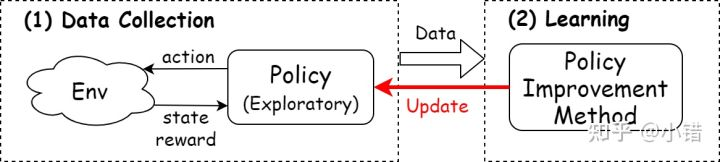
\includegraphics[scale=0.5]{pix/exploration.jpg}
\caption{Two tasks of an RL algorithm}
%\label{fig:label}
\end{figure}

RL 算法中都需要做两件事:
\begin{itemize}
%\setlength{\itemsep}{0pt}
%\setlength{\parsep}{0pt}
\setlength{\parskip}{0pt}
\item[(1)]
收集数据(Data Collection):与环境交互,收集学习样本; 
\item[(2)]
学习(Learning)样本:学习收集到的样本中的信息,提升策略。
\end{itemize}

RL 算法的最终目标是学习每种状态下最优的动作,而在训练过程中,
收敛(到最优策略 $\pi^*$)前的当前策略 $\pi$ 并非最优,所以它提供的动作并非最优。
为了找到动作空间里潜在的最优动作,算法必须尝试当前策略 $\pi$ 认为的非最优的动作,
因此 RL 算法中的策略需要有随机探索(Exploration)的能力。

%+++++++++++++++++++++++++++++++++++++++++++
\subsection{策略如何做到随机探索}

RL算法中的策略分为确定性(Deterministic)策略与随机性(Stochastic)策略:
\begin{itemize}
%\setlength{\itemsep}{0pt}
%\setlength{\parsep}{0pt}
\setlength{\parskip}{0pt}
\item
确定性策略 $\pi(s)$ 为一个将状态空间 $S$ 映射到动作空间 $A$ 的函数,即 
$\pi : S \rightarrow A$。它本身没有随机性质,因此通常会结合 $\epsilon-\text{greedy}$ 
或往动作值中加入高斯噪声的方法来增加策略的随机性。
\item
随机性策略 $\pi(A_t | S_t)$ 是条件为 $S_t \in S$ 情况下,动作 $A_t$ 的条件概率分布。
它本身带有随机性,获取动作时只需对概率分布进行采样即可。
\end{itemize}

为了不让思路凌乱,这里仅讨论 $Q$ 函数构造的确定性策略及其增加随机性的方式。
用 $Q$ 函数构造确定性策略是一种常见的策略形式,其具体方式是:
\begin{equation}\label{eq_argmax_policy_construction}
\pi(s)= \arg \underset{a}{\max}\; Q(s, a) 
\end{equation}

即选取 $Q$ 值最大的动作为最优动作。(注意:一般只有在动作空间离散的情况下采用这种策略,
若动作空间连续上式中的最大化操作需要经过复杂的优化求解过程。)

可用 $\epsilon-\text{greedy}$ 方法将上述确定性策略改造成具有探索能力的策略:
$$
\pi_\epsilon(s)=\begin{cases}
\arg\max_a\; Q(s,a), &\text{with probability } 1 - \epsilon \\
\text{random action}, &\text{with probability } \epsilon
\end{cases}
$$

即,以 $\epsilon$ 的概率选择随机动作(Exploration),以 $1 - \epsilon$ 
的概率按照确定性策略 $\pi(s)$ 选取动作。


\subsection{Example of a Policy}

Let's now see an example of policy in a practical scenario, 
to better understand how it works. In this example, an agent 
has to forage food from the environment in order to satisfy 
its hunger. It then receives rewards on the basis of the 
fruit it eats:

\begin{figure}[h]

\centering
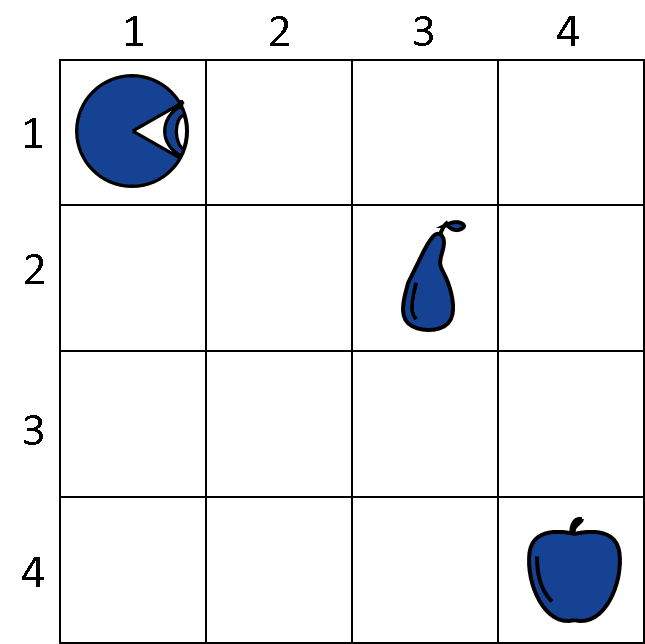
\includegraphics[scale=0.5]{pix/example1.png}
\caption{example figure}
%\label{fig:label}
\end{figure}

The internal state of the agent corresponds to its location 
on the board, in this case, $s_t = (x,y)$ and $s_0 = (1,1)$. 
The action space, in this example, consists of four possible 
behaviors: $A = \text{up, down, left, right}$. The probability 
matrix $P$ contains all pairwise combinations of states 
$(s, s')$ for all actions in $A$. It's Bernoulli-distributed, 
and looks like this:
\begin{align*}
P_{\text{down}}( (1,1), (1,2) ) &= 1; \\
P_{\text{down}}( (1,1), (1,3) ) &= 0; \\
... ; \\
P_{\text{up}}( (4,4), (4,3) ) &= 1
\end{align}

The reward function $R$ is defined in this manner. If it's 
in an empty cell, the agent receives a negative reward of 
$-1$, to simulate the effect of hunger. If instead, the 
agent is in a cell with fruit, in this case, $(3,2)$ for 
the pear and $(4,4)$ for the apple, it then receives a 
reward of $+5$ and $+10$, respectively.

The reward function $R$ thus looks like this:
\begin{align*}
R(\text{No fruit}) &= -1 \\
R(\text{Pear}) &= +5 \\
R(\text{Apple}) &= +10
\end{align}

The simulation runs for an arbitrary finite number of time 
steps but terminates early if the agent reaches any fruit.



\subsection{Evaluation of the Policies}

The agent then considers two policies $\pi_1$ and $\pi_2$. 
If we simplify slightly the notation, we can indicate a 
policy as a sequence of actions starting from the state of 
the agent at $s_0$:

\begin{itemize}
%\setlength{\itemsep}{0pt}
%\setlength{\parsep}{0pt}
\setlength{\parskip}{0pt}
\item[1.]
$\pi_1 = \text{down, right, right} \to \text{Pear}$

\item[2.]
$\pi_2 = \text{right, right, right, down, down, down} \to \text{Apple}$

\end{itemize}


\begin{figure}[h]
\centering
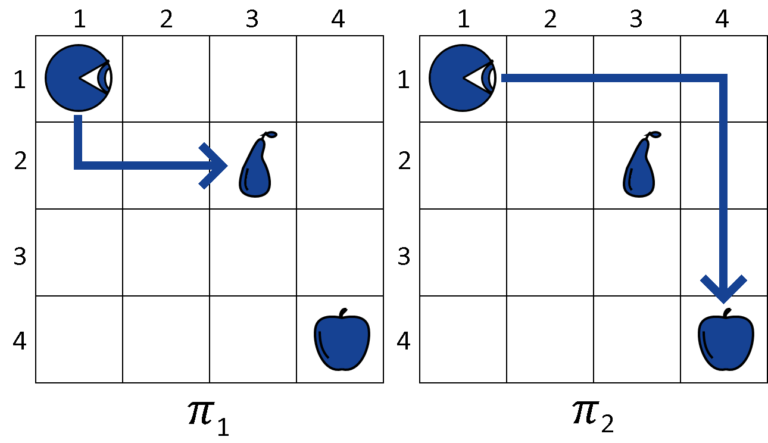
\includegraphics[scale=0.3]{pix/example1_1.png}
\caption{example figure1}
%\label{fig:label}
\end{figure}

The agent then has to select between the two policies. 
By computing the utility function $U$ over them, the 
agent obtains:

\begin{align*}
U(\pi_1) &= -1-1+5 = +3 \\
U(\pi_2) &= -1-1-1-1-1+10 = +5
\end{align}

\begin{figure}[h]

\centering
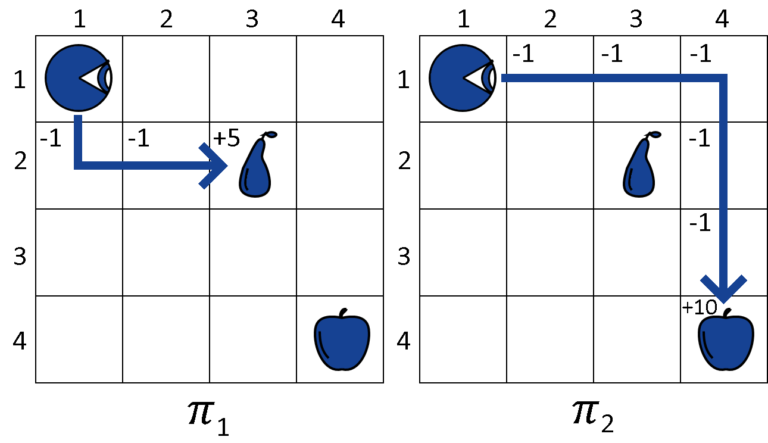
\includegraphics[scale=0.3]{pix/example1_2.png}
\caption{example figure2}
%\label{fig:label}
\end{figure}

The evaluation of the policies suggests that the utility 
is maximized with $\pi_2$, which then the agent chooses 
as its policy for this task.


%+++++++++++++++++++++++++++++++++++++++++++
% Policy Types
%-------------------------------------------

\section{Policy Types}

{\bf Deterministic and Stochastic Policies Explained} \cite{Loevenich2021}

行为策略是用来与环境互动产生数据的策略,即在训练过程中做决策;而目标策略在行为策略产生的
数据中不断学习、优化,即学习训练完毕后拿去应用的策略。百官(锦衣卫)就是行为策略,
去收集情况或情报,给皇帝(目标策略)做参考来学习,当皇帝收集到的情报越多,能做的决策就越优。

为了解决强化学习问题中的exploitation(利用) 和 exploration (探索),我们可以利用一个
策略(行为策略)来保持探索性,提供多样化的数据,而不断地优化另一个策略(目标策略)。
On-policy 的目标策略和行为策略是同一个策略,其好处就是简单粗暴,直接利用数据就可以优化
其策略,但这样的处理会导致策略其实是在学习一个局部最优,因为On-policy的策略没办法很好的
同时保持既探索又利用;而Off-policy将目标策略和行为策略分开,可以在保持探索的同时,更能求
到全局最优值。但其难点在于:{\bf 如何在一个策略下产生的数据来优化另外一个策略?}

From the previous section we know that a policy is a description of how an 
agent behaves given its current state and the goal. In this section, 
we will discuss Policy Types: Deterministic Policies and Stochastic Policies.

{\bf Deterministic Policies:} In a deterministic policy, the action taken 
at each state is always the same. This can be implemented using a lookup 
table or decision tree. In this case, we denote it is denoted by $\mu$:
$$
a_t = \mu(s_t)
$$

{\bf Stochastic Policies:} A stochastic policy, on the other hand, produces 
different actions from one instance to the next, but these are still chosen 
according to some fixed probabilities. The stochastic policy is denoted by 
$\pi$:
$$
a_t \sim \pi(\cdot | s_t)
$$

Because the policy is essentially the agent's brain, it's not unusual to 
replace "policy" with "agent," such as when someone says, "The agent is 
attempting to maximize reward."

In deep RL, we deal with parameterized policies: policies that produce 
computable functions that are dependent on a set of parameters (for example, 
the weights and biases of a neural network) that may be adjusted to modify 
the outcome using some optimization algorithm. 

Categorical and diagonal Gaussian policies are the two most frequent types 
of stochastic policies in deep RL. Categorical policies can be applied in 
discrete action regions, while diagonal Gaussian policies are appropriate for 
continuous action regions. 

{\bf Categorical Policy:} A categorical policy is a stochastic policy that 
favors either one or zero actions in each state, with equal probabilities 
assigned to all possible action choices.

{\bf Diagonal Gaussian Policy:} On the other hand, Diagonal Gaussian policies 
take any number of actions from zero to infinity and distribute them according 
to a diagonal Gaussian distribution. This means that in any given state, the 
agent can select from many different actions with equal probabilities assigned 
to all possible action choices.

The two most important computations for employing and training stochastic 
policies are:

\begin{itemize}
%\setlength{\itemsep}{0pt}
%\setlength{\parsep}{0pt}
\setlength{\parskip}{0pt}
\item[1)]
Sampling actions from the policy,

\item[2)]
Comparing log-likelihoods of various actions.
\end{itemize}

We'll go through how to implement these for both categorical and diagonal 
Gaussian policies in the following. 



%+++++++++++++++++++++++++++++++++++++++++++
% On-Policy vs Off-Policy
%-------------------------------------------

\section{On-Policy VS Off-Policy}

\cite{Sagar2020}

古时候,优秀的皇帝都秉持着“水能载舟 亦能覆舟”的思想,希望能多了解民间百姓的生活。
皇帝可以选择通过微服出巡,亲自下凡了解百姓生活(On-policy)。虽然眼见为实,
但毕竟皇帝本人分身乏术,掌握情况不全;因此也可以派多个官员去了解情况,
而皇帝本人则躺在酒池肉林里收听百官情报即可(Off-policy)。

Comparing reinforcement learning models for hyperparameter optimization is 
an expensive affair, and often practically infeasible. So the performance of 
these algorithms is evaluated via on-policy interactions with the target 
environment. These interactions of an on-policy learner help get insights 
about the kind of policy that the agent is implementing.

An off-policy, whereas, is independent of the agent's actions. It figures 
out the optimal policy regardless of the agent's motivation. For example, 
Q-learning is an off-policy learner.

On-policy methods attempt to evaluate or improve the policy that is used to 
make decisions. In contrast, off-policy methods evaluate or improve a policy 
different from that used to generate the data.

Here is a snippet from Richard Sutton's book on reinforcement learning where 
he discusses the off-policy and on-policy with regard to Q-learning and 
SARSA respectively:

\subsection{Off-policy}

In Q-Learning, the agent learns optimal policy with the help of a greedy 
policy and behaves using policies of other agents. Q-learning is called 
off-policy because the updated policy is different from the behavior policy, 
so Q-Learning is off-policy. In other words, it estimates the reward for 
future actions and appends a value to the new state without actually following 
any greedy policy.

\subsubsection{Off-policy 将收集数据当做一个单独的任务}

RL 算法中需要带有随机性的策略对环境进行探索获取学习样本,一种视角是:off-policy 
的方法将收集数据作为 RL 算法中单独的一个任务,它准备两个策略:behavior policy and
target policy。行为策略是专门负责学习数据的获取,具有一定的随机性,
总是有一定的概率选出潜在的最优动作。
而目标策略借助行为策略收集到的样本以及策略提升方法提升自身性能,并最终成为最优策略。
Off-policy 是一种灵活的方式,如果能找到一个“聪明的”行为策略,总是能为算法提供最合适的样本,
那么算法的效率将会得到提升。

the learning is from the data off the target policy(引自《Reinforcement 
Learning An Introduction》)。也就是说 RL 算法中,数据来源于一个单独的用于探索的策略
(不是最终要求的策略)。以 Q-Learning 为例,它的算法流程如下:

\begin{figure}[h]
\centering
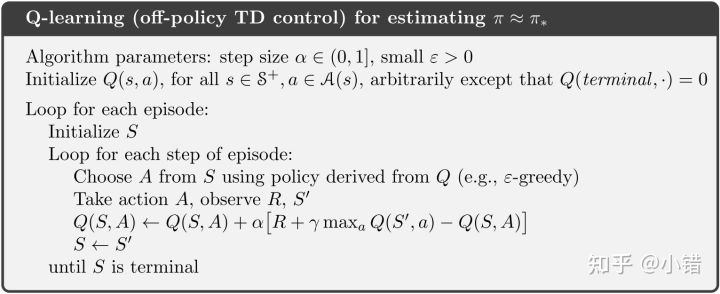
\includegraphics[scale=0.5]{pix/qlearning.jpg}
\caption{Q-Learning}
%\label{fig:label}
\end{figure}

算法流程图不够直观,将算法中的值函数更新式改写成另外一种形式后将算法用图描绘。

\begin{figure}[h]
\centering
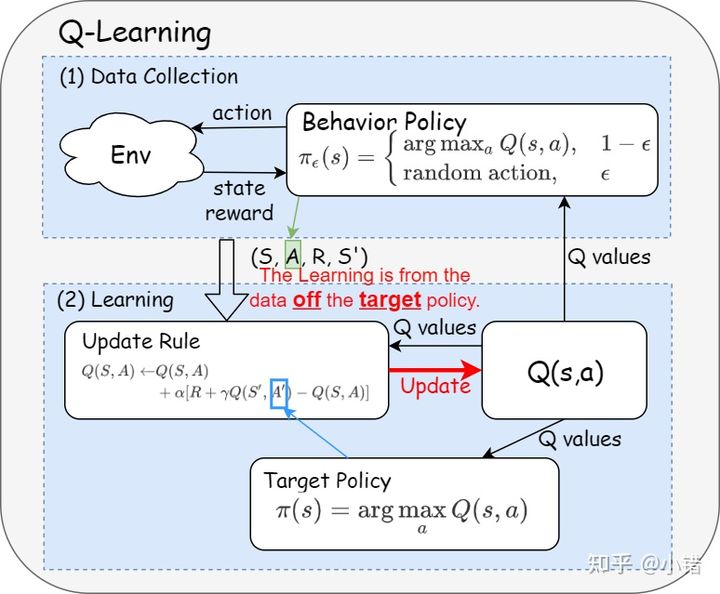
\includegraphics[scale=0.5]{pix/qlearning_flow.jpg}
\caption{Flow of Q-Learning}
%\label{fig:label}
\end{figure}

如图所示,$Q$-Learning 数据收集部分用的是由$Q$函数构造的
$\epsilon-\text{greedy}$策略 $\pi_\epsilon(s)$ (行为策略),而它的最终目标是
greedy 策略$\pi(s)$(目标策略)。$Q$函数更新规则(update rule)中的训练样本
$(S,\; A,\; R,\; S')$是由行为策略$\pi_\epsilon(s)$(而非目标策略)提供,
因此它是典型的 off-policy 方法。

\subsubsection{为什么有时候off-policy需要与重要性采样配合使用?}

重要性采样是用一个概率分布的样本来估计某个随机变量关于另一个概率分布的期望。

假设已知随机策略$\pi(a | s)$,现在需要估计策略$\pi$对应的状态值
$V^\pi$,但是只能用另一个策略$\pi'(a | s)$获取样本。对于这种需要用另外一个策略
的数据(off-policy)来精确估计状态值的任务,需要用到重要性采样的方法,具体做法是在对应
的样本估计量上乘上一个权重($\pi$与$\pi'$的相对概率),称为重要性采样率。

以off-policy Monte Carlo估计为例,它的步骤为:
\begin{itemize}
%\setlength{\itemsep}{0pt}
%\setlength{\parsep}{0pt}
\setlength{\parskip}{0pt}
\item[(1)]
由$\pi'$与环境交互生成一条样本轨迹:$(s_0,a_0,r_0,s_1,a_1,r_1,\dots,s_T,a_T,r_T)$,
$T(s)$表示轨迹样本中状态为$s$时间点的集合。$|T(s)|$为该集合的元素的总数量。
\item[(2)]
$t$时刻之后的轨迹序列关于$\pi$与$\pi'$的似然分别为
$\prod_{k=t}^T\pi(a_k|s_k)Pr(s_{k+1}|s_k, a_k)$与
$\prod_{k=t}^T\pi'(a_k|s_k)Pr(s_{k+1}|s_k, a_k)$,对应的重要性采样率为:
$$
\rho_t^T=\frac{\prod_{k=t}^T\pi(a_k|s_k)Pr(s_{k+1}|s_k, a_k)}{\prod_{k=t}^T\pi'(a_k|s_k)Pr(s_{k+1}|s_k, a_k)}
=\frac{\prod_{k=t}^T\pi(a_k|s_k)}{\prod_{k=t}^T\pi'(a_k|s_k)}
$$
\item[(3)]
$t$时刻之后的总回报为$G_t=\sum_{k=t}^T\gamma^{k-t}r_k$
\item[(4)]
按照MC方法估计状态s对应的状态值:
$$
V(s)=\frac{\sum_{t\in T}\rho_t^TG_t}{|T(s)|}
$$
\end{itemize}
最后再次强调,如果需要用off-policy方法估计/预测状态值或动作值时,需要用到重要性采样。

\subsubsection{为什么Q-Learning算法(或DQN)身为off-policy可以不用重要性采样?}

$Q^*(s,a)$ 为最优策略对应的$Q$函数,最优$Q$函数遵循如下最优贝尔曼等式:
$$
Q^*(s,a)=\sum_{s',r}Pr(s', r | s, a) [r + \gamma \max_{a'}Q^*(s', a')]
$$
{\bf $Q$-Learning的思想是从任意初始化的Q函数出发,以最优贝尔曼方程为标准调整$Q$函数。}
观察$Q$函数在第$n$轮更新时的更新式:
$$
Q_{n+1}(s, a) \leftarrow Q_n(s, a) + \alpha [r + \gamma \max_{a'}Q_n(s', a')
- Q_n(s, a)]
$$
可以看到它实际是以最优贝尔曼的估计量$r + \gamma\, \underset{a'}{\max}Q_n(s', a')$为目标(target),
让$Q_{n+1}(s, a)$尽量靠近该目标。需要注意到:{\bf 最优贝尔曼等式右侧的期望只与状态转移
分布有关而与策略无关,不论训练数据$(S,\; A,\; R,\; S')$来自于哪个策略,按照$Q$-Learning
的更新式更新都能使$Q$函数接近$Q^*(s,a)$。}因此,$Q$-Learning可以不采用重要性采样。
(DQN算法同理)

\subsubsection{重要性采样的数学说明}

为了能从行为策略$b$产生的样本回合(Episode)中评估(学习)策略$\pi$,我们要求当执行
$b$策略时,$\pi$中的每个动作都有一定概率发生,也就是$\pi(a|s)>0$时,必有
$b(a|s)>0$(逆命题不一定成立)。这种要求称为“包含”(Coverage)。在求最优策略的过程中,
目标策略$\pi$通常都是基于当前评估的价值函数$V$的贪婪策略(策略$\pi$的函数$V$的学习数据
来源于策略$b$,但并非直接利用$b$的$V$函数,后面会详细解释)。因此目标策略最终能收敛为
最优策略,而行为策略$b$则保持随机因而具有探索性。

几乎所有的off-policy都利用到一种技巧“Important Sampling”,这种技巧可以解决:
求解一个概率分布(Distribution)的期望值(Expect)时,用来求解该期望值的样本数据是由
另一个概率分布所产生。具体做法是:根据目标策略$\pi$和行为策略$b$分别所产生的相同某段序列
(这里我们把Episode中某一段称为Trajectory)的概率的比值来加权求和return(Return是MC
法中的一个样本序列(整个Episode)的总奖励),这个比值称为{\bf importance-sampling 
ratio}。(也就是把一段又一段的序列总价值根据importance-sampling ratio加权求和,
得到某个state的价值期望)
\begin{equation}\label{sate_gain_expectation}
\rho_t^{T-1}=\frac{\prod_{k=t}^{T-1}\pi(A_k|A_k)p(S_{k+1}|S_k, A_k)}{\prod_{k=t}^{T-1}b(A_k|A_k)p(S_{k+1}|S_k, A_k)}
=\frac{\prod_{k=t}^{T-1}\pi(A_k|S_k)}{\prod_{k=t}^{T-1}b(A_k|S_k)}
\end{equation}

【注意,上式只有当两个策略产生的由$t$到$T-1$的序列完全一样时,才能消掉转移概率。
(实际上排列顺序不一致但出现的转移情况一致也可以消掉转移概率)】

式中$\pi(A_k|S_k)$为策略$\pi$时的动作概率分布,$b(A_k|S_k)$为策略$b$时的动作概率分布。

虽然一个trajectory的发生可能性与环境的动态(即转移概率$p$)有关,但是通过比值可以消掉环
境的动态因素。因此importance-sampling ratio只由策略$b$、策略$\pi$和相应的序列所决定,
与MDP无关。 

因此,当我们评估(Estimate)在目标策略$\pi$下的奖励期望(Expected Return)时,
不能直接使用来自行为策略$b$产生的样本数据所计算得到的奖励期望$E[G_t|S_t]$,因为这样将不能
对样本数据进行平均求和而得到目标策略的价值函数。

\subsubsection{Thinking in variational method}

\begin{minipage}[t][2.5cm][t]{2em}
测试
\end{minipage}
行为策略似乎是在测试空间做添加噪声的处理,而目标策略似乎是在算子空间做逼近处理。
off-policy与on-policy只是选取了概率统计的方式来进行处理的算法选择而已。
%\begin{minipage}[c][2.5cm][t]{2em}
%测试2
%\end{minipage}

\subsection{On-policy}

SARSA (state-action-reward-state-action) is an on-policy reinforcement 
learning algorithm that estimates the value of the policy being followed. 
In this algorithm, the agent grasps the optimal policy and uses the same to 
act. The policy that is used for updating and the policy used for acting is 
the same, unlike in Q-learning. This is an example of on-policy learning.

An experience in SARSA is of the form $⟨S,A,R,S', A' ⟩$, which means that

\begin{itemize}
%\setlength{\itemsep}{0pt}
%\setlength{\parsep}{0pt}
\setlength{\parskip}{0pt}
\item
current state $S$, 
\item
current action $A$, 
\item
reward $R$, and 
\item
new state $S'$,
\item
future action $A'$. 

\end{itemize}

This provides a new experience to update from
$$
Q(S,A)\quad \text{to}\quad R + \gamma\, Q(S', A').
$$

on-policy的特点就是:the target and the behavior polices are the same。
也就是说on-policy里面只有一种策略,它既为目标策略又为行为策略。SARSA算法即为典型的
on-policy的算法,下图所示为SARSA的算法示意图,可以看出算法中只有一种策略,
训练的数据来自于它。

\begin{figure}[h]
\centering
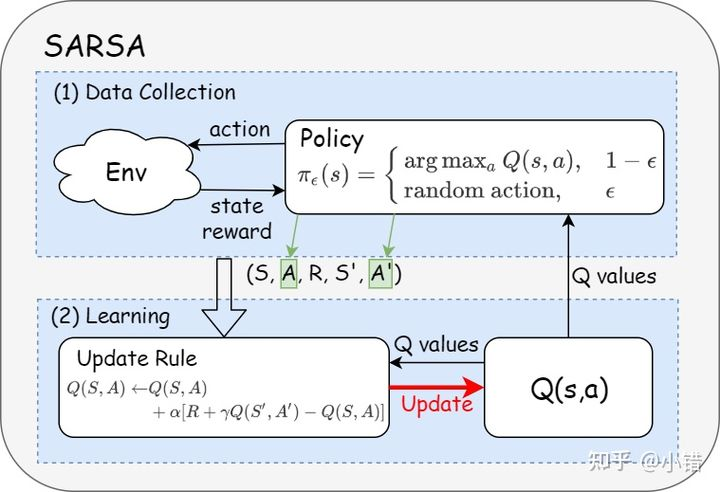
\includegraphics[scale=0.5]{pix/SARSA_flow.jpg}
\caption{Flow of SARSA algorithm}
%\label{fig:label}
\end{figure}

\subsubsection{SARSA算法(on-policy)像是在进行值函数估计,为什么能收敛到最优策略?}

更新式中用到的策略也是$\epsilon$-greedy算法。$\epsilon$的概率是用随机动作,
对策略的提升没有帮助;但另外有$1-\epsilon$的概率,按照
$\arg \underset{a}{\max}\, Q(s,a)$选取动作,即对策略进行提升。{\bf 可以发现
$\epsilon$-greedy策略是一种完全不同于用条件概率分布表示的策略,只要$\epsilon$较小,
它自带策略提升的功能。}


\subsection{Conclusion}

On-policy reinforcement learning is useful when you want to optimize the 
value of an agent that is exploring. For offline learning, where the agent 
does not explore much, off-policy RL may be more appropriate.

For instance, off-policy classification is good at predicting movement in 
robotics. Off-policy learning can be very cost-effective when it comes to 
deployment in real-world, reinforcement learning scenarios. The 
characteristic of the agent to explore and find new ways and cater for the 
future rewards task makes it a suitable candidate for flexible operations. 
Imagine a robotic arm that has been tasked to paint something other than 
what it is trained on. Physical systems need such flexibility to be smart 
and reliable. You do not want to hardcode use cases today. The goal is to 
learn on the go.

However, off-policy frameworks too are not without any disadvantages. 
Evaluation becomes challenging as there is too much exploration. These 
algorithms might assume that an off-policy evaluation method is accurate in 
assessing the performance. But agents fed with past experiences may act very 
differently from newer learned agents, which makes it hard to get good 
estimates of performance. 

Promising directions for future work include developing off-policy methods 
that are not restricted to success or failure of reward tasks, but extending 
the analysis to stochastic tasks as well.

For more information, check Richard Sutton's book.

% https://web.stanford.edu/class/psych209/Readings/SuttonBartoIPRLBook2ndEd.pdf

\begin{itemize}
%\setlength{\itemsep}{0pt}
%\setlength{\parsep}{0pt}
\setlength{\parskip}{0pt}
\item
off-policy的最简单解释: the learning is from the data off the target policy。
\item
On/off-policy的概念帮助区分训练的数据来自于哪里。
\item
Off-policy方法中不一定非要采用重要性采样,要根据实际情况采用(比如,需要精确估计值函数时
需要采用重要性采样;若是用于使值函数靠近最优值函数则不一定)。
\end{itemize}

%.............................
% 2.3.3
\subsection{What is the difference between Q-learning and SARSA?}

https://stackoverflow.com/questions/6848828/what-is-the-difference-between-q-learning-and-sarsa

\subsubsection{提问者自己的作答}

SARSA is on-policy while Q-learning is off-policy, but when looking at their 
formulas it's hard to see any difference between these two algorithms.

According to the book Reinforcement Learning: An Introduction 
(by Sutton and Barto \cite{Sutton1998}). In the SARSA algorithm, given a 
policy, the corresponding action-value function $Q$ (in the state $s$ and action 
$a$, at timestep $t$), i.e. $Q(s_t, a_t)$, can be updated as follows
$$
Q(s_t, a_t) = Q(s_t, a_t) + \alpha *(r_t + \gamma *Q(s_{t+1}, a_{t+1}) - Q(s_t, a_t))
$$
On the other hand, the update step for the Q-learning algorithm is the following
$$
Q(s_t, a_t) = Q(s_t, a_t) + \alpha *(r_t + \gamma *\max_aQ(s_{t+1}, a) - Q(s_t, a_t))
$$
which can also be written as
$$
Q(s_t, a_t) = (1-\alpha)*Q(s_t, a_t) + \alpha * (r_t+\gamma *\max_aQ(s_{t+1}, a))
$$
where $\gamma$ is the discount factor and $r_t$ is the reward received from 
the environment at timestep $t$.

Is the difference between these two algorithms the fact that SARSA only looks 
up the next policy value while Q-learning looks up the next maximum policy value?

The post writer has made a github repo
http://alexge233.github.io/relearn/
playing with Q-learning  and empirically understood what the difference is.
It all amounts to {\bf how you select your next best action}, which from an 
algorithmic standpoint can be a mean, max or best action depending on how 
you chose to implement it.

The other main difference is when this selection is happening (e.g., online 
vs offline) and how/why that affects learning. If you are reading this in 
2019 and are more of a hands-on person, playing with a RL toy problem is 
probably the best way to understand the differences.

One last {\bf important} note is that both Suton & Barto as well as Wikipedia 
often have mixed, confusing or wrong formulaic representations with regards 
to the next state best/max action and reward:
\begin{emp_box}
$r(t+1)$
\end{emp_box}
is in fact
\begin{emp_box}
$r(t)$
\end{emp_box}
Hope this helps anyone ever getting stuck at this.

\subsubsection{Another answer}

When I was learning this part, I found it very confusing too, so I put 
together the two pseudo-codes from R.Sutton and A.G.Barto hoping to make 
the difference clearer(见下面图\ref{fig:SARSA}).
\begin{figure}[h]
\centering
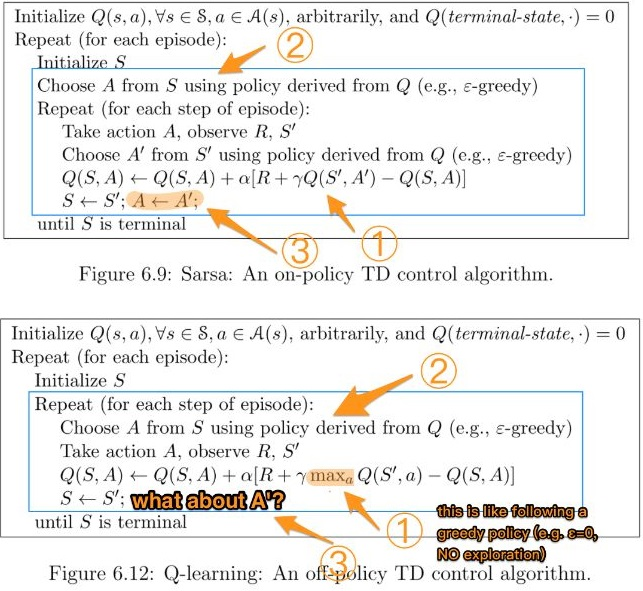
\includegraphics[scale=0.7]{pix/sarsa.jpg}
\caption{SARSA: An on-policy TD control algorithm}
\label{fig:SARSA}
\end{figure}

\noindent Blue boxes highlight the part where the two algorithms actually differ. 
Numbers highlight the more detailed difference to be explained later.

\begin{table}[htb]   
\begin{center}   
%\caption{title}  
%\label{table:1} 
\begin{tabular}{|c|c|c|}   
\hline    & \textbf{SARSA} & \textbf{Q-learning} \\   
\hline   Choosing $A'$ & $\pi$ & $\pi$  \\ 
\hline   Updating $Q$ & $\pi$ & $\mu$  \\  
\hline   
\end{tabular}   
\end{center}   
\end{table}

\noindent where $\pi$ is a $\epsilon$-greedy policy (e.g. $\epsilon > 0$ with 
exploration), and $\mu$ is a greedy policy (e.g. $\epsilon \equiv 0$, 
NO exploration).
\begin{itemize}
%\setlength{\itemsep}{0pt}
%\setlength{\parsep}{0pt}
\setlength{\parskip}{0pt}
\item[1.]
Given that $Q$-learning is using different policies for choosing next 
action $A'$ and updating $Q$. In other words, it is trying to evaluate 
$\pi$ while following another policy $\mu$, so it's an off-policy algorithm.
\item[2.]
In contrast, SARSA uses $\pi$ all the time, hence it is an on-policy algorithm.
\end{itemize}

\noindent {\bf More detailed explanation:}
\begin{itemize}
%\setlength{\itemsep}{0pt}
%\setlength{\parsep}{0pt}
\setlength{\parskip}{0pt}
\item[1.]
The most important difference between the two is how $Q$ is updated after 
each action. SARSA uses the $Q'$ following a $\epsilon$-greedy policy 
exactly, as $A'$ is drawn from it. In contrast, $Q$-learning uses the 
maximum $Q'$ over all possible actions for the next step. This makes it look 
like following a greedy policy with $\epsilon \equiv 0$, i.e. NO exploration 
in this part.
\item[2.]
However, when actually taking an action, $Q$-learning still uses the action 
taken from a $\epsilon$-greedy policy. This is why "Choose A ..." is inside 
the repeat loop.
\item[3.]
Following the loop logic in $Q$-learning, $A'$ is still from the 
$\epsilon$-greedy policy.
\end{itemize}

Congratulations for the beautiful graphics and pics. Years after I asked 
this question I came to realise that the state and action iteration, and 
the policy value iteration and update, are two different processes. Sadly, 
Sutton and Barto don't make this very clear. How you decide on actions 
affects the algorithms as you explained. Max action in $Q$-Learning usually 
implies choosing the action with next best $Q(s,a)$ e.g., greedy. In Sarsa 
this isn't the case, you either follow the policy (on-line) or you explore 
a new one depending on a random probability. Your description is spot on!

\subsubsection{Answers from Partagons and others(知乎)}

比如说现在有某个策略$\pi$,根据这个策略走到状态$s'$时应该采取动作$a'$。
\begin{itemize}
%\setlength{\itemsep}{0pt}
%\setlength{\parsep}{0pt}
\setlength{\parskip}{0pt}
\item[1)]
Sarsa更新$Q$值的方式是:
$$
Q(s,a) \leftarrow Q(s,a) + \alpha (R + \gamma Q(s',a') - Q(s,a))
$$
\noindent 更新值的时候是依据$a'$,也就是说确实采用了既有的策略$\pi$,所以叫on-policy

\item[2)]
$Q$-learning更新$Q$值的方式是:
$$
Q(s,a) \leftarrow Q(s,a) + \alpha (R + \gamma \max_aQ(s',a) - Q(s,a))
$$
\noindent 这里更新的时候没有用到$a'$啊,而是直接取了使$Q$值最大的那个动作$a$,
和既有的策略$\pi$是不一样的,所以叫off-policy
\end{itemize}

\begin{emp_box}
\indent 把on-policy翻译为同策略,off-policy翻译为异策略,比较好理解,指的是用来评价改进
的目标策略(target policy)与{\bf 学习过程中}做决策产生样本的行为策略(behavior 
policy)的异同。
\end{emp_box}




%+++++++++++++++++++++++++++++++++++++++++++
% 2.4 Why using behavior policy instead of target policy
%-------------------------------------------
\section{Why using behavior policy instead of target policy}

why to use different policy in order to build the action value 
function?

\begin{emp_box}
An advantage of this separation is that the target policy may 
be deterministic (e.g., greedy), while the behavior policy can 
continue to sample all possible actions.
\end{emp_box}

The more usual way of framing it is exploration vs 
exploitation. Theory tells you in standard MDPs that the 
optimal policy will be deterministic - each state has one 
"best" action that you should always take for optimal 
behaviour (sometimes more than one equivalent action, but 
in that circumstance you can always choose which one 
deterministically).

So you end up with some difficult issues using an on-policy 
control approach:
\begin{itemize}

\item
If you work with a single deterministic policy as your 
behaviour policy during learning, you will not learn enough 
about alternative behaviours in order to find better outcomes 
and improve the policy.

\item
If you work with a stochastic policy that covers all 
possible choices - to guarantee exploration - you know that 
can never be optimal. Careful manipulation of how the 
stochastic part varies (such as reducing $\epsilon$ in 
$\epsilon$-greedy policies) can get you arbitrarily close 
to a truly optimal policy, but then you are using the same 
parameters to manipulate both exploration rate and closeness 
to optimality of your learned policy, which means 
compromising between best exploration and the best end results.
\end{itemize}

\begin{emp_box}
What it makes it more interesting than an on policy method 
that only use a single policy?
\end{emp_box}


With off-policy learning, a target policy can be your best 
guess at deterministic optimal policy. Whilst your behaviour 
policy can be chosen based mainly on exploration vs 
exploitation issues, ignoring to some degree how the 
exploration rate affects how close to optimal the behaviour 
can get.

It is worth noting that some environments can be simple 
enough or stochastic enough with state transition and reward, 
that you can use a deterministic policy with and on-policy 
learner to explore and learn optimal control. However, you 
cannot rely on that in general, it would be more common that 
such an agent would stop learning at some point, far short 
of being optimal.


%+++++++++++++++++++++++++++++++++++++++++++
% 2.5 An example
%-------------------------------------------
\section{An example}

\begin{figure}[h]
\centering
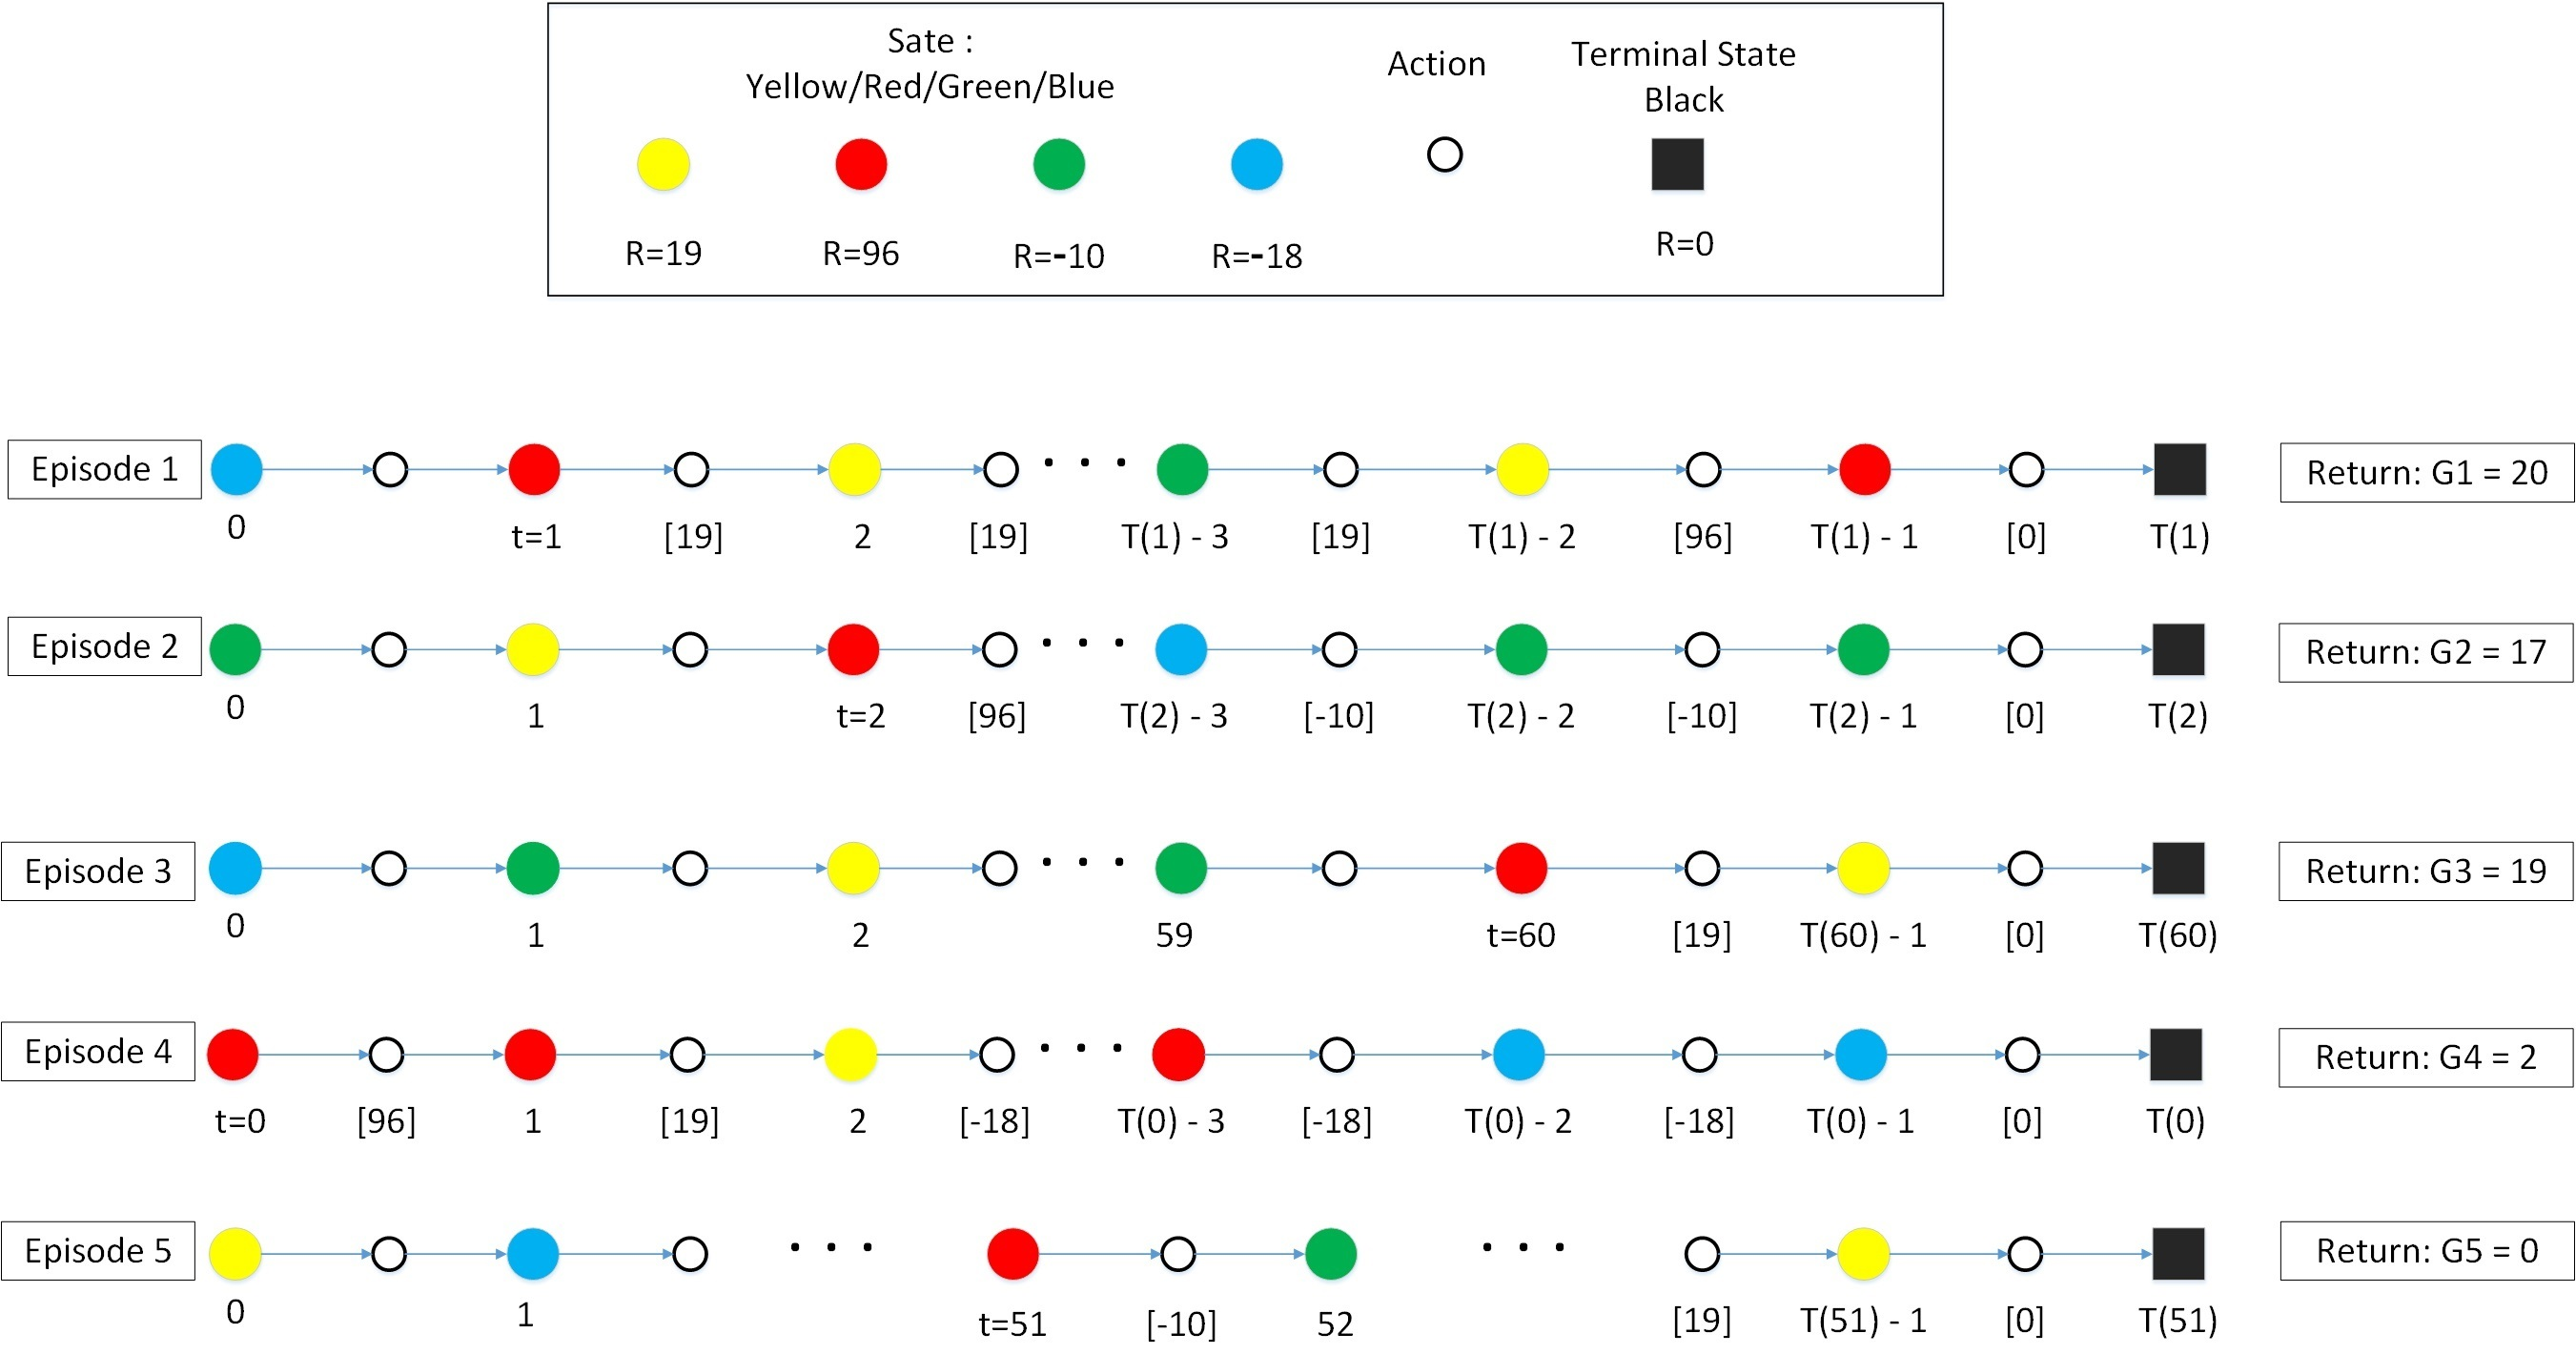
\includegraphics[scale=0.17]{pix/example.jpg}
\caption{An Example of Monte Carlo Methods with First-visit Technic}
%\label{fig:label}
\end{figure}

本例子基于Monte Carlo过程,环境的动态情况未知(即状态转移概率未知)。并采用
first-visit方法,即指定计算某一个状态(State)的价值时,只计算每个回合第一次出现
该状态(State)之后到结束的总奖励(Return)。

有五个状态:黄、红、绿、蓝、黑。其中黑状态为终止状态(Terminal)。在第一个框中每个
状态下面为即时奖励(Reward)。在此为了简化例子不具体列出动作,用一个空心环代替动作
集合的任一动作。当遇到黑色时就结束当前回合(Episode)。我们用$t$表示第一次遇到指定
状态的时间步,在本例中指定计算红色状态的价值(Red State Value),$T(t)$
表示一个回合中的终点的时间步。

\subsubsection{1. 采样}

基于行为策略$b$与环境互动,经过采样后,我们得到五个回合(省略部分为动作-状态序列)。

\subsubsection{2.计算每个样本回合的Return}

在这里取第三个回合(Episode 3)分析,假设在其省略序列部分没有出现红色,第一次遇到红色在
第60时间步(Time Step),则从此时开始计算后面的奖励。第61步为黄色,可得奖励19,第62步
为黑色,可得奖励0,并终止回合。经计算后该回合从第一个红色状态开始后得到的总奖励G3
(Return)为19。

其他回合也是这样处理算出每个回合的Return。(假设其他回合的省略部分随机出现除了黑色以外
的所有状态)

\subsubsection{3.计算行为策略b的红色状态的价值期望}

由Monte Carlo计算方法可知
$$
v_b(S_t=\text{Red})=E[G_t|S_t=\text{Red}]
=(G_1+G_2+G_3+G_4+G_5)/5 = 11.6
$$

11.6为在行为策略$b$下时,红色状态的价值(即Return的期望值)。在实际应用中,根据大数定理,
采样回合(Episode)的数量一般需要成千上万个,才能保证所计算的结果接近期望值。
On-policy中就是应用这个价值来进行学习、改善策略的,也即基于贪婪思想选取最大值的动作,
然后作为新的On-policy的策略。

\subsubsection{4. 计算目标策略$\pi$的红色状态的价值期望}

由于importance-sampling ratio 均可由公式\eqref{sate_gain_expectation}计算得到,所以这里未给出具体的动作及其在
相应策略下的概率以简化问题,因此在这里假设$\rho_1^{T(1)-1}$、$\rho_2^{T(2)-1}$、
$\rho_60^{T(60)-1}$、$\rho_0^{T(0)-1}$、$\rho_51^{T(51)-1}$分别为5,10,5,20,10。
有以下运算:
\begin{align*}
&\quad\ v_t(S_t=\text{Red}) \\
&= E[\rho_t^{T-1}G_t|S_t=\text{Red}] \\
&= (\rho_1^{T(1)-1}G_1 + \rho_2^{T(2)-1}G_2 + 
\rho_60^{T(60)-1}G_3 + \rho_0^{T(0)-1}G_4 + \rho_51^{T(51)-1}G_5)/5 \\
&= (5*20 + 10*17 +5*19 + 20*2 + 10*0) / 5 \\
&= 81
\end{align}

因此81为我们从由行为策略$b$产生的五个Episode中,所得到的目标策略$\pi$下的红色状态的价值
(即目标策略下的红色状态的Returne期望值)。然后根据该价值来学习,也即基于贪婪思想选取最大
值的动作,然后作为新的目标策略$\pi$。 

上述方法可称为普通的重要度采样,与之对应的还有加权重要度采样(本文不赘述,可在Sutton书中的
第五章查看)。前者在统计学意义上是无偏估计,但方差很大(比如在上述例子中11.6与81),后者则
是有偏估计(偏差逐渐收敛到0),方差也能收敛到零。

On-policy-与Off-policy的区别在于:更新价值所使用的方法是沿着既定的策略(on-policy)抑
或是新策略(off-policy)。

\cite{Sutton1998}
%\parencite{Sutton1998}


%+++++++++++++++++++++++++++++++++++++++++++
\section{An Introduction to Policy Gradient Methods}
%-------------------------------------------
% https://jmichaux.github.io/week2/

Basic reinforcement learning problems are often formulated as a {\bf Markov Decision Process} 
$ M = \lbrace S, A, R, P, \gamma \rbrace $, where $ S $ is the distribution of states, 
$ A $ is the set of actions the agent can take,  $ R = R(s, a) $ is the reward function, 
$ P $ are the state transition dynamics, and and $ \gamma $ is the discount factor. The goal is 
{\bf to find a policy $ \pi $ that maps states $ s \in S $ to optimal or near-optimal actions 
$ a \in A $}.

在强化学习中,有三个组成部分:演员(actor)、环境和奖励函数。其中环境和奖励函数不是我们可以控制的,
在开始学习之前就已经事先给定。演员里会有一个策略,它用来决定演员的动作。策略就是给定一个外界输入,
它会输出演员现在应该要执行的动作。我们唯一可以做的就是调整演员里面的策略,使得演员可以得到最大的奖励。

当我们将深度学习与强化学习相结合时,策略 $\pi$ 就是一个网络,用 $\theta$ 表示 $\pi$ 的参数。
演员根据概率的分布来决定它要采取的动作,概率分布不同,演员采取的动作也不同。简单来说,
策略的网络输出是一个概率分布,演员根据这个分布去做{\bf 采样},决定实际上要采取的动作是哪一个。


%+++++++++++++++++++++++++++++++++++++++++++
\subsection{Policy Gradients}


\subsubsection{Function Approximation}


我们知道可以通过方程 {\ref{eq_argmax_policy_construction}} 来构造确定性策略。
How do we do argmax when action space is large or continuous?

{\bf Idea}: Do Policy Improvement step with a Gradient Ascent instead

回顾在基于价值的方法(例如 DQN )中,使用价值函数近似将 $Q$-table 更新问题变成一个函数拟合问题,
相近的状态得到相近的输出动作,如下式,通过更新参数 $w$ 使得函数 $f$ 逼近最优 $Q$ 值。
$$
Q(s,a) \approx f(s,a; {\bf w})
$$
在 PG 算法中,因为策略是一个概率,不能直接用来迭代,所以我们采取类似的思路,将其转化为函数形式,
如下式所示,这时我们的目的则是使用带有 $\theta$ 参数的函数对策略进行近似,通过更新参数 $\theta$,
逼近最优策略。
$$
\pi(a|s) \approx \pi_\theta(s,a) = P(a|s, \theta)
$$
The reason that we write $\pi_\theta$ is that the $\theta$ refers to the parameters of 
function approximator, which for a deep neural net corresponds to the weights of the 
network.
现在有了策略函数,我们的目标当然是优化它,那么该如何知道优化后的策略函数的优劣呢。
大家肯定会想到需要一个可以优化的目标函数,我们让这个目标函数朝着最大值的方向去优化,
它的主要作用就是用来衡量策略的好坏程度。

与基于值函数来构造确定性策略不同,策略梯度算法是一种更为直接的方法,它让神经网络直接输出策略函数 
$\pi(s)$,即在状态 $s$ 下应该执行何种动作。对于非确定性策略,输出的是这种状态下执行各种动作的概率值,
即如下的条件概率:
$$
\pi(a|s) = p(a|s)
$$
所谓确定性策略,是只在某种状态下要执行的动作是确定即唯一的,而非确定性动作在每种状态下要执行的动作是随机的,
可以按照一定的概率值进行选择。这种做法的原理如下图\ref{fig:output_of_stochastic_policy}所示。

\begin{figure}[h]
\centering
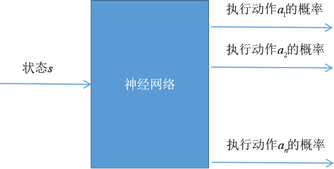
\includegraphics[scale=0.618]{pix/policy/output_of_stochastic_policy.png}
\caption{stochastic output.}
\label{fig:output_of_stochastic_policy}
\end{figure}
\noindent
此时的神经网络输出层的作用类似于多分类问题的 softmax 回归,输出的是一个概率分布,
只不过这里的概率分布不是用来进行分类,而是执行动作。至于对于连续型的动作空间该怎么处理,我们在后面会解释。

因此,如果构造出了一个目标函数 $L$,其输入是神经网络输出的策略函数 $\pi(a|s)$,通过优化此目标函数,
即可确定神经网络的参数 $\theta$,从而确定策略函数 $\pi(a|s;\theta)$。这可以通过梯度上升法实现
(与梯度下降法相反,向着梯度方向迭代,用于求函数的极大值)。训练时的迭代公式为:
$$
\theta_{t+1}=\theta_t + \alpha\nabla_\theta L(\theta_t)
$$
这里假设策略函数对参数的梯度 $\nabla_\theta\pi(a|s;\theta)$ 存在,从而保证 
$\nabla_\theta L(\theta_t)$。现在问题的核心就是如何构造这种目标函数 $L$,以及如何生成训练样本。
对于后者,采用了与 DQN 类似的思路,即按照当前策略随机地执行动作,并观察其回报值,以生成样本。

对于第一个问题,一个自然的想法是使得按照这种策略执行时的累计回报最大化,即构造出类似 $V$ 函数和 $Q$ 
函数这样的函数来。

Policy Gradient methods are a family of reinforcement learning algorithms that rely on optimizing 
a parameterized policy directly. As alluded to above, the goal of the policy is to maximize the 
total expected reward:
$$
\mathbb{E}_{\tau \sim p_\theta (\tau)} [R(\tau)]. \tag{1}
$$
Policy gradient methods have a number of benefits over other reinforcement learning methods. First, 
by optimizing the policy directly, it is not required that we also learn a value function (although 
we'll later see that learning a value function can help). Second, policy gradient methods can handle 
both discrete and continuous states and actions, making them well suited for high dimensional 
problems. This is in contrast to methods such as Deep $Q$-learning, which struggles in high 
dimensions because it assigns scores for each possible action.

In addition to their benefits, policy gradient methods also have a few drawbacks. By definition, 
policy gradient methods are on-policy. This means that they are only able to learn from data that 
was collected with the current policy. As a result, policy gradient methods are not very sample 
efficient. Another issue is that policy gradient methods are not guaranteed to converge to a global 
optimum, and solutions may get stuck in local optima. Lastly, policy gradient methods tend to suffer 
from high variance. However, even with these drawbacks, policy gradient methods such as TRPO and PPO 
are still considered to be the state-of-the art reinforcement learning algorithms.


\subsubsection{Policy Improvement with a Gradient Ascent}

\begin{itemize}
%\setlength{\itemsep}{0pt}
%\setlength{\parsep}{0pt}
\setlength{\parskip}{0pt}
\item[-]
We want to find the Policy that fetches the “Best Expected Returns”
\item[-]
Gradient Ascent on “Expected Returns” w.r.t params of Policy func
\item[-]
So we need a func approx for (stochastic) Policy Func: $\pi(s, a; {\bf \theta})$
\item[-]
In addition to the usual func approx for Action Value Func: $Q(s, a; {\bf w})$
\item[-]
$\pi(s, a; \theta)$ called {\bf Actor} and $Q(s, a; {\bf w})$ called {\bf Critic}
\item[-]
Critic parameters ${\bf w}$ are optimized w.r.t $Q(s, a; {\bf w})$ loss function $\min$
\item[-]
Actor parameters $\theta$ are optimized w.r.t Expected Returns $\max$
\item[-]
We need to formally define “Expected Returns”
\item[-]
But we already see that this idea is appealing for continuous actions
\item[-]
GPI(Generalized Policy Iteration) with Policy Improvement done as 
{\bf Policy Gradient (Ascent)}
\end{itemize}


\subsubsection{Advantages and Disadvantages of Policy Gradient approach}

\noindent{\bf Advantages:}
\begin{itemize}
%\setlength{\itemsep}{0pt}
%\setlength{\parsep}{0pt}
\setlength{\parskip}{0pt}
\item[-] 
Finds the best Stochastic Policy (Optimal Deterministic Policy,
produced by other RL algorithms, can be unsuitable for POMDPs)

\item[-] 
Naturally explores due to Stochastic Policy representation

\item[-] 
Effective in high-dimensional or continuous action spaces

\item[-] 
Small changes in $\theta$ $\Rightarrow$ small changes in $\pi$, and in state distribution

\item[-] 
This avoids the convergence issues seen in argmax-based algorithms

\end{itemize}


\noindent{\bf Disadvantages:}
\begin{itemize}
%\setlength{\itemsep}{0pt}
%\setlength{\parsep}{0pt}
\setlength{\parskip}{0pt}
\item[-] 
Typically converge to a local optimum rather than a global optimum

\item[-] 
Policy Evaluation is typically inefficient and has high variance

\item[-] 
Policy Improvement happens in small steps $\Rightarrow$ slow convergence

\end{itemize}


\subsubsection{“Expected Returns” Objective}

Now we formalize the “Expected Returns” Objective:
\begin{equation}\label{eq_er_objective}
J(\theta) = \mathbb{E}_\pi\left[ \sum_{t=0}^\infty \gamma^t \cdot R_{t+1} \right]
\end{equation}

Value Function $V^\pi(s)$ and Action Value function $Q^\pi(s, a)$ defined as:
\begin{align*}
V^\pi(s) &= \mathbb{E}_\pi\left[ 
\sum_{k=t}^\infty\gamma^{k-t}\cdot \mathcal{R}_{k+1} | \mathcal{S}_t = s
\right] \quad \text{for all } t=0,1,2,\ldots \\
Q^\pi(s,a) &= \mathbb{E}_\pi\left[  
\sum_{k=t}^\infty\gamma^{k-t}\cdot \mathcal{R}_{k+1} | \mathcal{S}_t = s, \mathcal{A}_t=a
\right] \quad \text{for all } t=0,1,2,\ldots 
\end{align}
Advantage Function:
$$
\mathcal{A}^\pi(s,a) = Q^\pi(s,a) - V^\pi(s)
$$
Also, $p(s\rightarrow s', t, \pi)$ will be a key function for us - it denotes the 
probability of going from state $s$ to $s'$ in $t$ steps by following policy $\pi$


%+++++++++++++++++++++++++++++++++++++++++++
\subsection{Policy Gradient Theorem}

\subsubsection{Discounted-Aggregate State-Visitation Measure}

折算——汇总状态——探寻测度

下面我们对公式 \ref{eq_er_objective} 进行变换:
\begin{align}
J(\theta) 
&= \mathbb{E}_\pi\left[ \sum_{t=0}^\infty \gamma^t \cdot \mathcal{R}_{t+1} \right] \notag \\
&= \sum_{t=0}^\infty \gamma^t \cdot \mathbb{E}_\pi[\mathcal{R}_{t+1}] \notag \\
&= \sum_{t=0}^\infty \gamma^t \cdot \sum_{s\in\mathcal{N}}\left(
\sum_{\mathcal{S}_0\in\mathcal{N}}p_0(\mathcal{S}_0)\cdot p(\mathcal{S}_0\rightarrow s,t,\pi)
\right) \cdot \sum_{a\in\mathcal{A}}\pi(s,a;\theta)\cdot\mathcal{R}_s^a \notag \\
&= \sum_{s\in\mathcal{N}}\left(\sum_{\mathcal{S}_0\in\mathcal{N}}\sum_{t=0}^\infty \gamma^t \cdot 
p_0(\mathcal{S}_0)\cdot p(\mathcal{S}_0\rightarrow s,t,\pi)
\right) \cdot \sum_{a\in\mathcal{A}}\pi(s,a;\theta)\cdot\mathcal{R}_s^a \notag \\
&= \sum_{s\in\mathcal{N}}\rho^\pi(s)
\cdot \sum_{a\in\mathcal{A}}\pi(s,a;\theta)\cdot\mathcal{R}_s^a
\end{align}
where $\rho^\pi(s) = \sum_{\mathcal{S}_0\in\mathcal{N}}\sum_{t=0}^\infty \gamma^t \cdot 
p_0(\mathcal{S}_0)\cdot p(\mathcal{S}_0\rightarrow s,t,\pi)$  is the key function
(for PG) we'll refer to as Discounted-Aggregate State-Visitation Measure.


\subsubsection{Policy Gradient Theorem (PGT)}

\begin{theorem}
\begin{equation}
\nabla_\theta J(\theta) = \sum_{s\in\mathcal{N}}\rho^\pi(s)
\cdot \sum_{a\in\mathcal{A}}\nabla_\theta\pi(s,a;\theta)\cdot Q^\pi(s,a)
\end{equation}
\end{theorem}

\begin{itemize}
%\setlength{\itemsep}{0pt}
%\setlength{\parsep}{0pt}
\setlength{\parskip}{0pt}
\item[-]
Note: $\rho^\pi(s)$ depends on $\theta$, but there's no $\nabla_\theta\rho^\pi(s)$ term 
in $\nabla_\theta J(\theta)$

\item[-]
Note: $\nabla_\theta\pi(s,a;\theta) = \pi(s,a;\theta)\cdot\nabla_\theta\log\pi(s,a;\theta)$

\item[-]
So we can simply generate sampling traces, and at each time step, calculate $(\nabla_\theta
\log\pi(s,a;\theta))\cdot Q^\pi(s,a)$ (probabilities implicit in paths)

\item[-]
Note: $\nabla_\theta\log\pi(s,a;\theta)$ is Score function (Gradient of log-likelihood)

\item[-]
We will estimate $Q^\pi(s,a)$ with a function approximation $Q(s,a;{\bf w})$

\item[-]
We will later show how to avoid the estimate bias of $Q(s,a;{\bf w})$

\item[-]
This numerical estimate of $\nabla_\theta J(\theta)$ enables {\bf Policy Gradient Ascent}

\item[-]
Let us look at the score function of some canonical $\pi(s,a;\theta)$

\end{itemize}



%+++++++++++++++++++++++++++++++++++++++++++
\subsection{The objective}

In deriving the most basic policy gradiant algorithm, we seek the optimal policy 
$ \color{Red}{\pi^*} $
that will maximize the total expected reward:
$$
\pi^{\ast} = \underset{\pi}{\operatorname{argmax}} \mathbb{E}_{\tau \sim p_{\theta}(\tau)}[R(\tau)] 
$$
where
\begin{align*}
\tau &= (s_1, a_1, \dots, s_T, a_T ) \\
R(\tau) &= \sum_{t=1}^{T}r(s_t, a_t) \\
p_{\theta}(\tau) &= p_{\theta}(s_1, a_1, ..., s_T, a_T). 
\end{align}

\begin{equation*}
\underbrace{p_{\theta}(s_1, a_1, ..., s_T, a_T)}_{p_{\theta}(\tau)} = p(s_1)
\prod_{t=1}^T p_\theta(a_t|s_t) p(s_{t+1}|s_t, a_t)
\end{equation}

\begin{align*}
\theta^{\ast} = \underset{\theta}{\operatorname{argmax}} \mathbb{E}_{\tau \sim p_{\theta}(\tau)}
\left[\sum_t r(s_t, a_t)\right] 
\end{align}

The {\bf trajectory} $ \tau $ is a sequence of states and actions experienced by the agent, 
so $\tau$ is just a shorthand for $s_1, a_1, s_2, a_2$, etc up until $s_T, a_T$.
$ R(\tau) $ is the {\bf return}, and {\bf $p_\theta(\tau)$ is referring to this distribution 
over trajectory $\tau$}. Or we can say $ p_\theta (\tau) $ is the probability of observing 
that particular sequence of states and actions, and the reason that it has a {\bf subscript 
$\theta$} is of course because it is influenced by the policy. It is important to note that 
$p_\theta (\tau)$ is a function of both the environment transition dynamics and the policy 
$ \pi $.

Since the policy $ \pi $ is parameterized by $ \theta $, finding the optimal policy 
$ \pi^* $ is equivalent to finding the optimal parameter vector $ \theta^{\ast} $:
\begin{align*}
\theta^{\ast} = \underset{\theta}{\operatorname{argmax}} \mathbb{E}_{\tau \sim p_{\theta}(\tau)}[R(\tau)] 
\end{align}
For the infinite horizon case the above formula can be writte as:
\begin{align*}
\underset{\text{infinite horizon case}}
{\theta^{\ast} = \underset{\theta}{\operatorname{argmax}} \mathbb{E}_{(s,a) \sim p_{\theta}(s,a)}[r(s,a)] 
}
\end{align}
For the finite horizon case we can write:
\begin{align*}
\underset{\text{finite horizon case}}
{\theta^{\ast} = \underset{\theta}{\operatorname{argmax}} \sum_{t=1}^T \mathbb{E}_{(s_t,a_t) 
\sim p_{\theta}(s_t,a_t)}[r(s_t,a_t)] 
}
\end{align}


\subsubsection{The infinite horizon case}

In this case, we can define our objective $ J(\theta) $ to be the total expected reward:
\begin{align*}
J(\theta) = \mathbb{E}_{\tau \sim p_\theta(\tau)}[R(\tau)] 
\end{align}

One way to optimize this objective is to take the derivative and then use gradient ascent. 
The calculation of the gradient goes as follows:
\begin{eqnarray}
\nabla J(\theta) &=&  \nabla \mathbb{E}_{\tau \sim p_\theta (\tau)}[R(\tau)]  \tag{8} \\
&=& \nabla \int  p_\theta(\tau) R(\tau) \mathrm{d\tau}  \tag{9} \\
&=& \int \nabla  p_\theta (\tau) R(\tau) \mathrm{d\tau}  \tag{10} \\
&=& \int p_\theta (\tau) \nabla log p_\theta (\tau) R(\tau) \mathrm{d\tau}  \tag{11} \\
&=& \mathbb{E}_{\tau \sim p_\theta (\tau)}[\nabla log p_\theta (\tau) R(\tau)]  \tag{12}
\end{eqnarray}


\subsubsection{The finite horizon case}

In this subsubsection let's just stick to the more convenient and simple finite horizon 
case. Let's talk about how we can actually optimize the subjective, how we can maximize 
the expected value of the total reward under the trajectory distribution induced by the 
policy $\pi_\theta$.

\begin{align*}
\theta^{\ast} = \underset{\theta}{\operatorname{argmax}} 
\underbrace{\mathbb{E}_{\tau \sim p_{\theta}(\tau)} \left[\sum_t r(s_t, a_t)\right]}_{J(\theta)}
\end{align}

\begin{align}
J(\theta) = \mathbb{E}_{\tau \sim p_{\theta}(\tau)} \left[\sum_t r(s_t, a_t)\right]
\approx& \frac{1}{N}\underset{\uparrow}{\sum_i}\sum_t r(s_{i,t}, a_{i,t}) \label{finite_horizon_J_theta}\\
&\text{sum over samples from }\pi_\theta \notag
\end{align}

Before we actually get into the whole maximization thing, let's try to think about something 
even more basic. How do we even evaluate this objective. how do we obtain an estimate of 
this expected value, if we do not know the transition distribution, we do not know the 
initial state distribution, we just have the world to interact with our policy.

How we can obtain an estimate for this expected value?
One of the ways that you can estimate an expectation, is that you can {\bf generate samples 
from the distribution under which the expectation is taken, and then averaged together the 
values of the quantity inside the expectation over those samples}. So the distribution is 
$P_\theta(\tau)$, the quantity of interest is the sum of the rewards over the trajectories. 
So one of the ways you can estimate that expectation is to obtain samples from $P_\theta(\tau)$, 
and the way that you can obtain those samples is by actually using your policy to act in 
the world. So if your policy controls a car driving on that cliff, just drive the car 50 
times, average the total reward over those 50 trials, and that's your estimate of the 
expected value of the total reward. It's a very simple way to obtain an estimate of an 
expected value, and we'll actually use this sampling based estimator multiple times in 
this subsection, not just to obtain the value for the objective, but also to actually 
figure out how to improve it.

\begin{figure}[h]
\centering
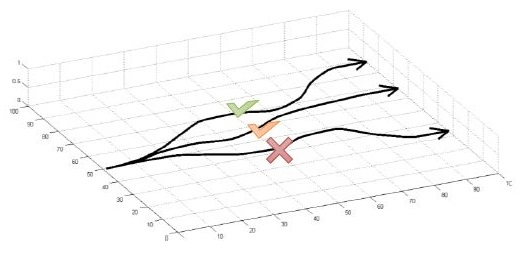
\includegraphics[scale=0.618]{pix/policy/steps_in_trajectories.jpg}
%\caption{Soft state value}
%\label{fig:label}
\end{figure}

So for notational convenience, $J(\theta)$ refers to this whole expectation. so $J(\theta)$ 
is basically the objective of reinforcement learning as a function of the policy parameters 
$\theta$. So $J(\theta)$ is equal to this expectation, and We can approximate it using 
samples. So when you see me write an equation like this, that just means I drew capital and 
samples, and I'm summing over all those samples of the quantity inside the expectation, 
which is the sum over time of the reward. So you generate some samples {\bf evaluate the 
total reward of each of those sample trajectories by summing together the rewards along all 
the time steps in those trajectories}. So maybe the green one is the best one, the red one 
is the worst one, and the orange one is somewhere in the middle, average those together, 
and that gives you an unbiased estimate of the expected reward of your policy. The 
subscript $i$ indexes over the samples. So this sum over $i$ from $i$ equals $1$ to capital 
$N$. So that lets us evaluate the objective.


%+++++++++++++++++++++++++++++++++++++++++++
\subsection{Direct Policy Differentiation}

Now let's talk about actually trying to maximize that objective discussed in the last 
subsection. So hopefully all of you know that if you calculate a gradient, then you can take 
a step in the direction of that gradient to increase the function value, take a step in the 
direction of the negative gradient to decrease the function value. Since we are using 
rewards, we'd like to maximize it, if we had costs, we would minimize it. So here since we 
want to maximize the quantity what we want to do is calculate the gradient, and take a step 
in the direction of the gradient. 

\begin{align*}
J(\theta) = \mathbb{E}_{\tau \sim \pi_\theta(\tau)}[R(\tau)] 
\end{align}

So for notational convenience, again if you see me write some $p_\theta$ or $\pi_\theta$ 
that denotes the distribution over trajectories, unfortunately we are here a little 
inconsistent $p_\theta(\tau)$ and $\pi_\theta(\tau)$ mean exactly the same thing. so don't 
worry about that, We'll fix those later, and $R(\tau)$ is just shorthand for the total 
reward over the trajectory $\tau$. 
\begin{align*}
J(\theta) = \mathbb{E}_{\tau \sim \pi_\theta(\tau)}
\underbrace{[R(\tau)]}_{\sum_{t=1}^Tr(s_t,a_t)}
\end{align}
So if you see something of $\tau$, that just denotes the sum in the case of rewards, or 
the product in the case of distributors. So we can write out an expectation like the following, 
\begin{align*}
J(\theta) = \mathbb{E}_{\tau \sim p_\theta(\tau)}
\underbrace{[R(\tau)]}_{\sum_{t=1}^Tr(s_t,a_t)} = \int p_\theta(\tau)R(\tau)d\tau
\end{align}
as an integral of the probability of that trajectory times the reward of that trajectory. 

And now if we want to calculate the derivative, we're going to try to differentiate this 
thing, so $J(\theta)$ is equal to this integral.
\begin{align*}
\nabla_\theta J(\theta) 
= \int \nabla_\theta  p_\theta (\tau) R(\tau) \mathrm{d\tau} 
\end{align}
so for the derivative, since integrals are linear, and I can put the gradient operator 
inside of it. what I really want is the gradient with respect to $\theta$ of $p_\theta(
\tau)$ times $R(\tau)$. now this quantity might at first seem a little daunting to obtain, 
because $p_\theta(\tau)$ contains inside of it the unknown initial state distribution, 
and the unknown transition distribution. So we need to do a little bit of kind of calculus 
magic to really get this quantity. and there's a very convenient identity that we can 
exploit that makes us very straightforward to get.

\begin{emp_box}
a convenient identity
\begin{align}
\label{eq_convenient_identity}
\textcolor{cyan}{p_\theta(\tau)\nabla_\theta\log p_\theta(\tau)}
= p_\theta(\tau)\frac{\nabla_\theta p_\theta(\tau)}{p_\theta(\tau)}
= \textcolor{blue}{\nabla_\theta p_\theta(\tau)}
\end{align}
\end{emp_box}
\noindent
So this is the identity, if you have a quantity like this, $p_\theta(\tau)$ times 
$\nabla_\theta\log p_\theta(\tau)$, then you can look up the equation for the derivative of 
a logarithm in a calculus textbook, and find out the derivative of a logarithm can be 
written as the derivative of the quantity that you're taking the logarithm of, which is 
$p_\theta(\tau)$, divided by that quantity which is $p_\theta(\tau)$. so 
$p_\theta(\tau)\nabla_\theta\log p_\theta(\tau)$ can be written as 
$p_\theta(\tau)\nabla_\theta\log p_\theta(\tau)$ divided by $p_\theta(\tau)$, and that's 
quite nice, because now the denominator here cancels with this quantity, and you're just 
left with $\nabla_\theta\log p_\theta(\tau)$. 

so grad $p_\theta(\tau)$ is what we've got 
over here, so we can substitute the left hand side of this equation, and turn that integral 
into the integral over $\tau$ of $p_\theta(\tau)$, $\nabla_\theta\log p_\theta(\tau)$, 
times $R(\tau)$. 

\begin{align*}
\nabla_\theta J(\theta) 
&= \int \textcolor{blue}{\nabla_\theta  p_\theta (\tau)} R(\tau) \mathrm{d\tau}  \\
&= \int \textcolor{cyan}{p_\theta (\tau) \nabla \log p_\theta (\tau)} R(\tau) \mathrm{d\tau}  \\
&= \mathbb{E}_{\tau\sim p_\theta(\tau)}\left[ \nabla_\theta\log p_\theta(\tau)R(\tau) \right] 
\end{align}
and this is now very convenient for us, because this integral has a $p_\theta(\tau)$ in 
the front of it, which means that it can also be written out as an expectation. So the 
derivative of $J_\theta$ can be written again as an expectation with respect to 
$p_\theta(\tau)$ of $\nabla_\theta\log p_\theta(\tau)R(\tau)$. now we're not quite out of 
the woods yet, because we still need to figure out what this $\nabla_\theta\log p$ actually 
is equal to.

So here we're going to bring back our equation for the distribution over trajectories. So 
this is the $p_\theta(\tau)$, and what it's equal to:
\begin{equation}
\label{eq_pg_p_theta_trajectories}
%\label{eq_pg_p_theta_trajectories_s}
\underbrace{p_{\theta}(s_1, a_1, ..., s_T, a_T)}_{p_{\theta}(\tau)} = p(s_1)
\prod_{t=1}^T p_\theta(a_t|s_t) p(s_{t+1}|s_t, a_t)
\end{equation}
(此公式在后面公式(\ref{eq_pg_p_theta_trajectories_s})还要使用)
and because we're after $\nabla_\theta\log p_\theta(\tau)$, we take the logarithm of both 
sides, now when you take the logarithm of a product, you get a sum of logarithms:
\begin{equation*}
\textcolor{cyan}{\log p_\theta(\tau)} = \textcolor{blue}{\log p(s_1) + \sum_{t=1}^T\log p_\theta(a_t|s_t)
+ \log p(s_{t+1}|s_t, a_t)}
\end{equation}
So if we take the $\log$ of both sides, we get $\log p_\theta(\tau)$ is equal to this huge 
thing, but this huge thing basically consists of three types of log transition probabilities, 
and $\log$ policy probabilities. So let's take that whole thing, and substitute that in 
there for our $\log p_\theta$. We're trying to take the gradient of this whole thing. So we 
don't really care about this quantity, we care about the gradient of this quantity. and of 
course because we have a sum, we can push the gradient operator inside the sum. 
\begin{align*}
\nabla_\theta J(\theta) 
&= \mathbb{E}_{\tau\sim p_\theta(\tau)}\left[ \nabla_\theta 
\textcolor{cyan}{\log p_\theta(\tau)}R(\tau) \right] \\
&= \mathbb{E}_{\tau\sim p_\theta(\tau)} \nabla_\theta\left[ 
\textcolor{blue}{\log p(s_1) + \sum_{t=1}^T\log p_\theta(a_t|s_t)
+ \log p(s_{t+1}|s_t, a_t)} \right] R(\tau)
\end{align}
So what $\nabla_\theta\log p(s_1)$ is equal to? zero. It's equal to zero because theta does 
not affect the probability of starting an initial State, regardless of which policy We pick, 
the universe will not change how its initial States for us. what is the derivative with 
respect to theta of $\log p(s_{t+1}|s_t, a_t)$, again zero. yeah so regardless of how you 
choose to buy or not buy lottery tickets, the probability of winning the lottery is not 
altered by your policy, that's determined by the universe. So random transitions are 
unaffected by $\theta$, initial state probabilities are not affected by $\theta$, so both of 
these cancel out. and we're just left with the $\log p_\theta$ terms, which are actually 
the only terms in the sum: 
\begin{align}
\label{eq_pg_gradient_of_log_p_trajectory}
\nabla_\theta\log p_\theta(\tau) = \sum_{t=1}^T \nabla_\theta\log p_\theta (a_t | s_t)
\end{align}
(后面 (\ref{eq_pg_off_policy_deducing}) 还要用到这个公式)
that we know, because that's our policy. So we can rewrite the 
gradients of the policy like this, 
\begin{align*}
\nabla_\theta J(\theta) 
= \mathbb{E}_{\tau\sim p_\theta(\tau)} \left[\left( 
\sum_{t=1}^T\nabla_\theta\log p_\theta(a_t|s_t) \right)
\left( \sum_{t=1}^Tr(s_t,a_t) \right)\right]
\end{align}
removing all the terms whose derivative is $0$, and leaving just the 
$\nabla_\theta\log p_\theta$ terms.


%+++++++++++++++++++++++++++++++++++++++++++
\subsection{Evaluating the policy gradient}

Now we have something very convenient, because we have a bunch of terms here, which we 
can evaluate because the policy is actually known to us, we have a bunch of rewards here, 
that we can evaluate. And all of this is taken in expectation under $p_\theta(\tau)$. So 
now how can we estimate this policy gradient? It's going to be very similar to how we 
evaluated the objective value before. Just like before we evaluated our reinforcement 
learning objective value by generating samples, by actually running our policy in the 
world, to get an estimate of an expectation in this form. now we'll do exactly the same 
thing, only on those samples. So, recall equation \ref{finite_horizon_J_theta}, in the case 
of finite horizon we have:
\begin{align*}
J(\theta) = \mathbb{E}_{\tau \sim p_{\theta}(\tau)} \left[\sum_t r(s_t, a_t)\right]
\approx \frac{1}{N}\sum_i\sum_t r(s_{i,t}, a_{i,t}) 
\end{align}
we won't just sum together and average the rewards as above, we sum 
together rewards and sum together these $\nabla_\theta\log p_\theta(\tau)$, multiply 
them, and then average that:
\begin{align*}
\nabla_\theta J(\theta) 
&= \mathbb{E}_{\tau\sim p_\theta(\tau)} \left[\left( 
\sum_{t=1}^T\nabla_\theta\log p_\theta(a_t|s_t) \right)
\left( \sum_{t=1}^Tr(s_t,a_t) \right)\right] \\
&\approx \frac{1}{N}\sum_{i=1}^N
\left( \sum_{t=1}^T\nabla_\theta\log p_\theta(a_{i,t}|s_{i,t}) \right)
\left( \sum_{t=1}^T r(s_{i,t}, a_{i,t}) \right)
\end{align}

So in order to evaluate the policy gradient, we basically use the same ideas before, 
using samples. So we generate some samples, evaluate their rewards, also evaluate 
their $\nabla_\theta\log p$, and then average those together. So this is an equation 
that we can actually implement in a computer to estimate the policy gradient using $N$ 
samples. and then once we've evaluated the gradients, then all we do is we modify our 
parameter values by taking the old parameters plus some learning rate times the 
gradient, and that implements gradient ascent. in practice, you can use other more 
powerful optimizers, but this is kind of the basic version.
$$
\theta \leftarrow \theta + \alpha\nabla_\theta J(\theta)
$$

\begin{figure}[h]
\centering
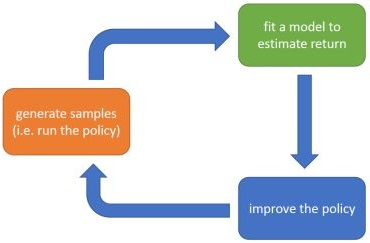
\includegraphics[scale=0.618]{pix/policy/policy_gradient_processing_flow.jpg}
%\caption{Soft state value}
%\label{fig:label}
\end{figure}

\noindent{\bf Q:} 
How do we pick $N$, and is a somehow related to the horizon $T$. 

\noindent{\bf A:} 
The answer is that in practice we always choose $N$ heuristically. we discuss 
some rules of thumb for how to choose $N$ as a hint needs to be a bit bigger than what 
you're used to in deep learning in terms of the theory, there is some variance analysis 
that can be done that relates $N$ to $T$. we won't cover in this section, but there is 
some references on item we could discuss that afterwards.

\noindent{\bf Q:} 
How do you make sure that the trajectory you get actually match the probabilities that 
you want, because you want this expectation to be under $p_\theta(\tau)$.

\noindent{\bf A:} 
The answer is that if you actually run your policy, the assumption in reinforcement 
learning is that the process that generates a trajectory matches the distribution. So 
when you basically request the environment please let me run my policy, it'll put you 
in a state sample from $p(s_1)$, then you pick the first action from your policy, and 
then you assume that the environment will then generate a sample from $P(s_2|s_1,a_1)$, 
if this is not true, then basically but this isn't gonna work. we will discuss what 
happens if you have samples from other distributions later on, though there are a few 
tricks there.

\noindent{\bf Q:} 
Why is the reward of $\tau$ not dependent on $\theta$?

\noindent{\bf A:} 
Remember that the policy is actually a probability distribution. So the policy doesn't 
just give you a one specific action for every state, $t$ actually gives you a probability 
distribution over actions given States, once you've actually sampled those actions, 
you have States and actions, you can plug those into the reward, the reward only depends 
on the states and actions. so if you alter the probability of the actions, then the 
expected reward will change, and that's actually already accounted for by these gradient 
terms out front. another way to think about this, is if you think back to the lecture 
from last week when I talked about how non-smooth functions, can still have smooth 
expectations, this is basically the same thing. so the example I had last week with 
falling off the cliff versus not falling, whether there was a probability the falling 
action that was given by theta, if you go back to the slides from last week, you'll see 
that there the equation for the reward was theta times reward for falling plus one minus 
theta times reward for not falling. So even though the reward was non smooth, the whole 
expectation is smooth in theta.

So let's come back to the anatomy of a reinforcement learning algorithm. So last week I 
talked about how every reinforcement learning algorithm consists of three parts, 
generation of samples, fitting a model or estimating a return, and improving the policy. 
and this algorithm does do all three of those things. 

\begin{figure}[h]
\centering
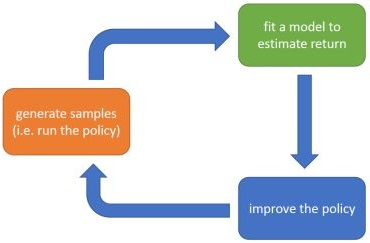
\includegraphics[scale=0.8]{pix/policy/policy_gradient_processing_flow.jpg}
\caption{Three parts of policy gradient algorithm}
%\label{fig:label}
\end{figure}

\begin{align*}
\nabla_\theta J(\theta) 
\approx \textcolor{orange}{\frac{1}{N}\sum_{i=1}^N}
\left( \sum_{t=1}^T\nabla_\theta\log p_\theta(a_{i,t}|s_{i,t}) \right)
\textcolor{green}{\left( \sum_{t=1}^T r(s_{i,t}, a_{i,t}) \right)}
\end{align}

$$
\textcolor{blue}{\theta \leftarrow \theta + \alpha\nabla_\theta J(\theta)}
$$

So the orange box is when you sample from your policy to get those samples from 
$p_\theta(\tau)$, the model here is very simple, the model just amounts to summing 
together your rewards, later on we'll actually see that we can replace the sum with 
more sophisticated estimators, so right now the green box is basically a summation 
operator, later on we'll see that we can use more fancy neural network learning methods 
to replace this piece. and then the blue box, the part where you actually improve your 
policy is just this gradient assent line. So you just take your gradient and take a step 
in the direction of their gradient, and that improves your policy as soon as you do that, 
of course you need to generate more samples.

\begin{emp_box}
Loop of REINFORCE algorithm:
\begin{itemize}
%\setlength{\itemsep}{0pt}
%\setlength{\parsep}{0pt}
\setlength{\parskip}{0pt}
\item[1.]
sample $\{\tau^i\}$ from $\pi_\theta(a_t|s_t)$ (run it on the robot)

\item[2.]
$\nabla_\theta J(\theta) \approx \sum_i(\sum_t\nabla_\theta\log\pi_\theta(a_t^i|s_t^i))
(\sum_tr(s_t^i, a_t^i))$

\item[3.]
$\theta \leftarrow \theta + \alpha\nabla_\theta J(\theta)$
\end{itemize}
\end{emp_box}

So using this derivation, we can actually already describe one of the most basic 
reinforcement learning algorithms which appropriately now what's called REINFORCE, the 
way that the REINFORCE algorithm works is that you {\bf sample a set of trajectories from 
your policy} by literally running that policy in the environment, then you {\bf estimate the 
policy gradient} using those samples, basically using this equation up here. and then 
you {\bf take a gradient step in the direction of that gradient which improves your policy}. 
So this is the REINFORCE algorithm, if someone says I trained my policy with REINFORCE, 
this is what they mean. only not really, because if you actually code this up, it won't 
work. So what we're going to talk about from here on out is how to actually make it work. 
But first we'll get a little bit more in-depth understanding of what it's doing. yes we'll 
find out, so stick around for the second half to find out the the surprise ending to this 
story. But before we find out why it doesn't work, let's try to understand it a little 
bit better.

\begin{align*}
\nabla_\theta J(\theta) 
\approx \frac{1}{N}\sum_{i=1}^N
&\left( \sum_{t=1}^T 
\underset{\textcolor{blue}{\uparrow}}{\textcolor{red}{\nabla_\theta\log p_\theta}}
(a_{i,t}|s_{i,t}) \right)
\left( \sum_{t=1}^T r(s_{i,t}, a_{i,t}) \right) \\
&\text{\qquad\textcolor{blue}{what is this?}}
\end{align}
What is $\nabla_\theta\log p$, and if we understand what $\nabla_\theta\log p_\theta(\tau)$ 
is, maybe that can help us implement it. So let's think of a kind of a practical example, 
maybe we have our driving policy, so images go in, steering commands come out and we have 
a $\pi_\theta(a|s)$, if we have a discrete action space, maybe it's just like turn left, 
turn right or drive straight, then we might implement $\pi_\theta(a|s)$ as a neural net 
that outputs the logics for categorical distribution. then you have a softmax layer on top, 
and that basically gives you probabilities over the three actions. So that's a very 
standard design that you could use for example for a neural network classifier, and that 
basically implements $\pi_\theta(a|s)$. So then the gradients of the $\log$ probabilities 
would just be obtained directly from your automatic differentiation software.


%+++++++++++++++++++++++++++++++++++++++++++
\subsection{Comparison to maximum likelihood}

It's kind of illustrative to consider how this compares to standard supervised learning. 
So when we do supervised learning, we're really doing maximum likelihood estimation. So 
the objective for maximum likelihood estimation kind of the supervised learning setup 
that we had before. Its gradient can be written out like this, so the gradient for 
maximum likelihood is just the sum over all your samples, I'll assume that my arranged 
in trajectories. So I also have some overtime steps, and in there I have the gradient 
of the log probability of the action that was taken in the data given the state that was 
in the data. So this is just supervised learning maximum likelihood. and if you look at 
the policy gradient, you'll see that they're actually quite similar, except that the 
policy gradient multiplies those $\nabla_\theta\log\pi_\theta$ by these total rewards. 
and this is actually quite a useful fact to know, because when we actually go to 
implement the policy gradient, we can implement it in a very similar way, as how we 
implement maximum likelihood training.

Policy gradient:
\begin{align*}
\nabla_\theta J(\theta) 
\approx \frac{1}{N}\sum_{i=1}^N
\left( \sum_{t=1}^T \nabla_\theta\log p_\theta(a_{i,t}|s_{i,t}) \right)
\left( \sum_{t=1}^T r(s_{i,t}, a_{i,t}) \right)
\end{align}
Maximum likelyhood:
\begin{align*}
\nabla_\theta J_{ML}(\theta) 
\approx \frac{1}{N}\sum_{i=1}^N
\left( \sum_{t=1}^T \nabla_\theta\log p_\theta(a_{i,t}|s_{i,t}) \right)
\end{align}

\begin{figure}[h]
\centering
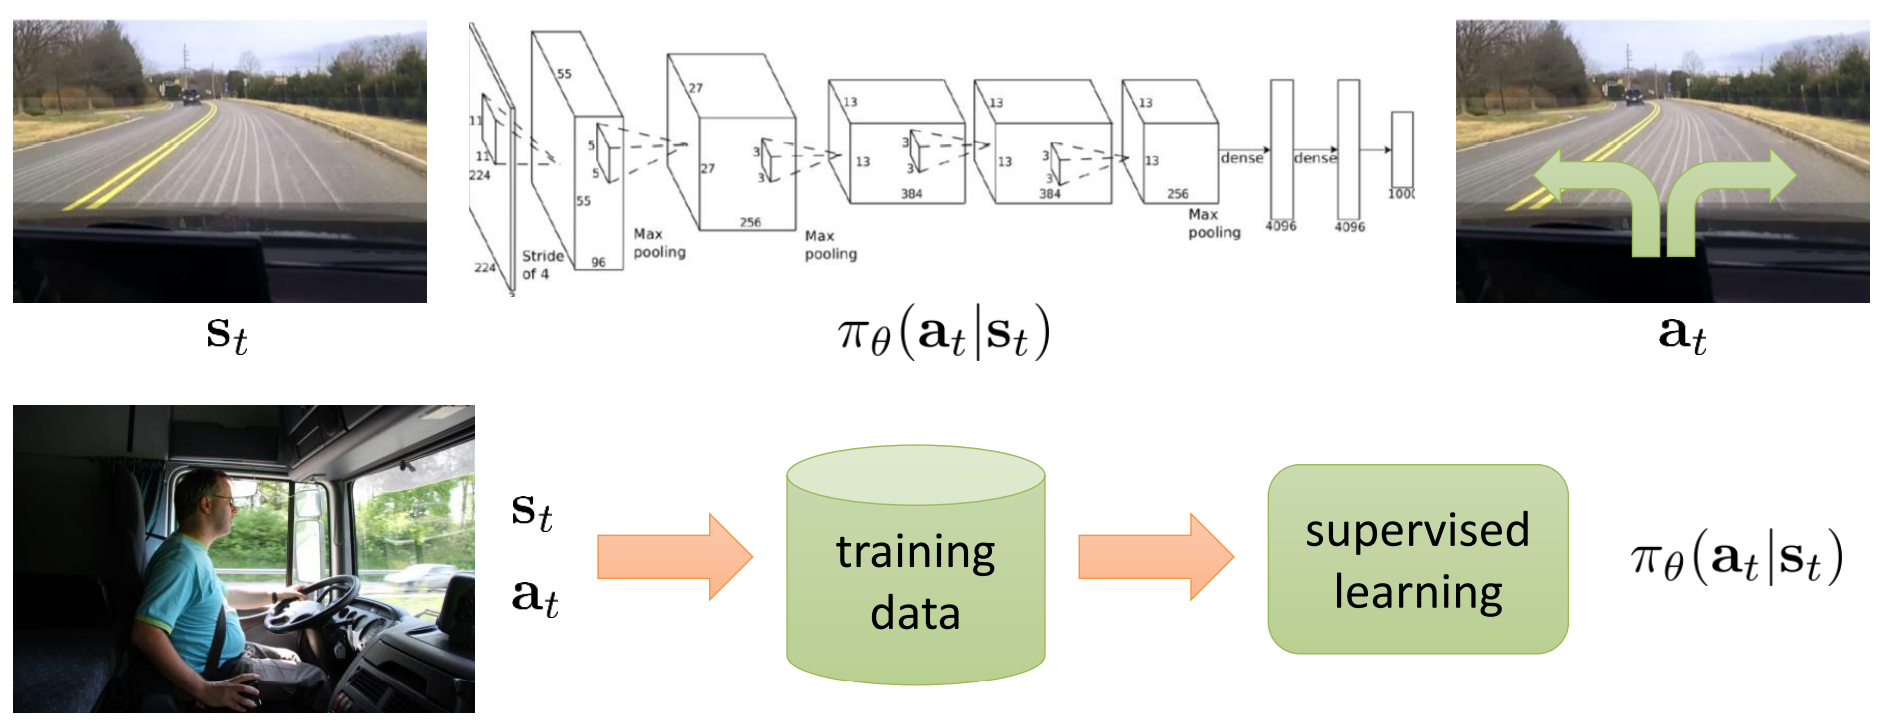
\includegraphics[scale=0.382]{pix/policy/pg_mle.png}
\caption{comparison to supervised learning}
%\label{fig:label}
\end{figure}

\subsubsection{Gaussian policies}

Let's go through another example, this was for continuous actions. So you could imagine 
using policy gradient to train a little simulated robot, in this case to run around. 
Now this simulated robot is going to have continuous actions not discrete actions. So we 
need $p_\theta(a|s)$ to define a distribution over some continuous value, a very popular 
choice is to use a {\bf multivariate normal distribution}.
$$
p_\theta(a_t|s_t) = \mathcal{N}\left(f_{\text{neural network}}(s_t); \Sigma\right)
$$
So in a multivariate normal distribution, {\bf your policy is you know maybe its mean is 
defined by some neural network, its covariance might also be defined by some neural 
network}, but for now I'll just say the {\bf covariance is constant for simplicity}. and 
{\bf theta represents the parameters of this neural network}.
$$
\log p_\theta(a_t|s_t) = -\frac{1}{2}\parallel f(s_t)-a_t \parallel_\Sigma^2 + \text{const}
$$
So if you write out the {\bf log probability}, this is just the equation for the log 
probability of a normal distribution, where {\bf everything that doesn't depend on the mean}, 
I've just kind of wrapped into this constant over here. So all the bits that depend on the 
neural network $f$, are just this piece, very simple equation.
$$
\nabla_\theta \log p_\theta(a_t|s_t) = 
-\frac{1}{2}\Sigma^{-1}\left(f(s_t)-a_t\right)\frac{df}{d\theta}
$$
and if you take the derivative of that with respect to theta, this is basically the 
equation you get. So you can work this out on paper at home. hopefully I didn't make a 
mistake, this is the the grad log PI theta for a multivariate normal distribution, 
where the mean is parameterized by this function $f$. okay now of course you don't 
actually have to do this by hand, typically if you use automatic differentiation 
software like Tensorflow or Pytorch, it'll do this calculation for you, but this is just 
to kind of make it more concrete, and to see that there's a relatively simple equation 
you can drive for these things in terms of the derivatives of some deterministic 
function. any questions about this, yeah exactly, so this is just the quadratic form in 
Sigma inverse, yeah this is just literally like the Wikipedia equation for the 
multivariate normal distribution.

\subsubsection{What did we just do?}

So that's kind of the mathematics of it. but let's talk also a little bit about the 
intuition of what's going on here. It sort of seemed like we did a bunch of mathematic 
trick, we ended up with some funny formulas, 
\begin{align*}
\nabla_\theta J(\theta) 
\approx \frac{1}{N}\sum_{i=1}^N
\left( \sum_{t=1}^T \nabla_\theta\log p_\theta(a_{i,t}|s_{i,t}) \right)
\left( \sum_{t=1}^T r(s_{i,t}, a_{i,t}) \right)
\end{align}
\begin{align*}
\tau_i &= (s_{i,1}, a_{i,1}, \dots, s_{i,T}, a_{i,T} ) \\
R(\tau_i) &= \sum_{t=1}^{T}r(s_{i,t}, a_{i,t}) \\
\nabla_\theta\log p_\theta(\tau_i) &= 
\sum_{t=1}^T \nabla_\theta\log_\theta p_\theta(a_{i,t} | s_{i,t})
\end{align}
(上面最后一个公式应该在 mle 中进行说明,因为二者后面都要用到)those funny formulas implement gradient 
asent, but what did we really do, like what is this? how does this algorithm actually 
change the policy in practice. So this is our policy gradient. 
\begin{align}
\label{eq_pg_compare_to_mle}
%\label{eq_pg_baselines_1}
\nabla_\theta J(\theta) 
\approx \frac{1}{N}\sum_{i=1}^N
\underbrace{\nabla_\theta\log p_\theta(\tau_i)}_{\sum_{t=1}^T \nabla_\theta\log_\theta p_\theta(a_{i,t} | s_{i,t})}
R(\tau_i)
\end{align}
(后面为了美观经常将 $R$ 写为 $r$,例如公式(\ref{eq_pg_baselines_1}),)
and just looking at the 
form of this equation, you can kind of maybe imagine that what it's going to do, is going 
to take the gradient. So the gradient of $\log p_\theta(\tau)$ basically points in the 
direction that will increase the probability of the trajectory $\tau$. so if I change my 
parameters in the direction of grad log $p_\theta(\tau)$ for a specific trajectory 
$\tau_i$. I will make $\tau_i$ more probable. So if I multiply those gradients by 
$R(\tau_i)$, it kind of seems like what I'm doing, is I'm making the high-reward 
trajectories more probable, and the lower-reward trajectory is less probable. So compared 
to the maximum likelihood, 
\begin{align*}
\nabla_\theta J_{ML}(\theta) 
\approx \frac{1}{N}\sum_{i=1}^N
\nabla_\theta\log p_\theta(\tau_i)
\end{align}
gradient we just makes everything more probable. Maximum 
likelihood just takes all of your data, and just makes it more likely, this one multiplies 
it by our $\tau$ which means that things with bad rewards will actually be made less likely. 
So you can imagine that visually like this, you got trajectories, you evaluate their 
rewards, some of them are good, some of them are bad, some of them are in the middle.

Your policy induces a distribution over trajectories, so if you got those three 
trajectories, maybe this height field represents your distribution, you'll take the ones 
with the good rewards, and you'll increase their probabilities, take the ones with the bad 
rewards, and decrease their probabilities. and this will make the expected reward larger, 
because the good stuff got more likely, the bad stuff got less likely. So good stuff is more 
likely, bad stuff less likely. there's this essentially just a very fancy mathematical 
version to formalize trial and error learning, if you got it right do it more often, if you 
got it wrong do it less often. So this is basically the intuition behind this method.


%+++++++++++++++++++++++++++++++++++++++++++
\subsection{Partial observability}

Now let's come back to this partial observibility point, and here I'm going to ask a 
question, can I do policy gradients with partial observibility? 

\begin{figure}[h]
\centering
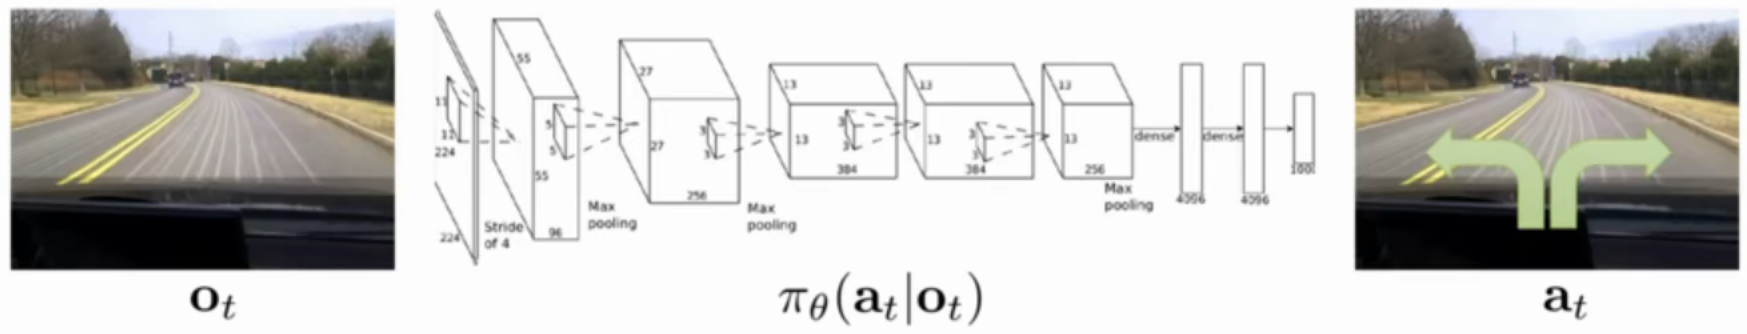
\includegraphics[scale=0.3]{pix/policy/pg_partial_observability.png}
%\caption{Histogram of Count Variable}
%\label{fig:label}
\end{figure}
\noindent
Okay, so that's interesting hypothesis right actions affect other actions. A world 
which does like having God abilities 
it knows everything to actually tell us what the next transition will be, so we still 
maintain our transition probabilities, even though we don't necessarily know the full 
state, so then in expectation it should still end up being about average.  
that's a reasonable way of looking at it. so the way that I look at it is that if you 
actually write out the equation like this, 
\begin{align*}
\nabla_\theta J(\theta) 
\approx \frac{1}{N}\sum_{i=1}^N
\left( \sum_{t=1}^T \nabla_\theta\log p_\theta(a_{i,t}|o_{i,t}) \right)
\left( \sum_{t=1}^T r(s_{i,t}, a_{i,t}) \right)
\end{align}
the assumption that the policy PI is 
conditioned on the Markovian state is not actually used anywhere by the policy. so the 
policy is just some function approximator that looks at something, and outputs an action 
distribution. and nowhere in this derivation, do we ever actually assume that the thing 
that the policy is conditioned on extra obeys the Markov property, now underneath all this 
there needs to be some system that obeys the Markov property, but we don't need to know 
what that system is, we just need to observe samples from that, and get rewards. the policy 
can be conditioned on whatever the heck we want. and of course any system can be turned 
into a Markovian system, if you just define your state as the full history of all 
observations you've seen so far. so you know, that might not be a very satisfying way to 
turn into Markovian system, but we don't care because we never even need to know what the 
state is, all wings do is to be able to generate samples, and get reward values for those 
samples, and evaluate our log pi which can be conditioned on whatever we want. {\bf So that's 
kind of a convenient fact with policy gradient that essentially we can just completely 
ignore all this stuff, and just do it on partial observability, this is the only algorithm 
that I'm going to cover over the next subsections}, which this is true, once we start 
introducing value functions, this will no longer be true.
\begin{emp_box}
{\bf Markov property is not actually used!}
\end{emp_box}

The sampler will still assume to sample states under the hood, like basically it's sort of 
this is not even an assumption about what's in your code as an assumption about how the 
universe works that when your policy interacts with the environment, that environment has 
a state, and it generates samples, samples of those states, but then what it shows you is 
the observations that are that are given rise according to those states. So you never 
actually see the states, you never know what they are, but they do exist there somewhere. 
and the nice thing is that any process, no matter how non Markovian it is can be written 
as a consequence of some underlying Markovian process defining a very trivial way just by 
setting the states to be the concatenation of observation histories.

So I was wondering a family would catch me on this, so this thing this $r$ still takes in 
$s$, and this is a little bit of a delicate point. so the actual assumption when an 
algorithm like this is implemented is that the environment will give your observations, 
and will actually also give you reward values, not reward functions just actual reward 
values, and those values do actually need to depend on states, but if they depend on 
observations you can equivalently just assume that your rewards are stochastic, because 
observations are stochastic consequence of your states. so you can say that a function of 
the observations is just to cast a consequence of your States. and then you're just 
assuming you don't observe deterministic reward values, but stochastic reward values, 
and with stochastic reward values you get another little expectation in there, and all 
the math still works out. 

{\bf Q:} So the question was are there methods that actually explicitly estimated 
emission probabilities

{\bf A:} absolutely and we'll talk about those later when we talk about model-based RL.

\begin{emp_box}
{\bf Can use policy gradient in partially observed MDP's without modification}
\end{emp_box}


%+++++++++++++++++++++++++++++++++++++++++++
\subsection{What is wrong with the policy gradient?}

So now I alluded to this before that if you actually code up REINFOECE the way I described, 
it won't work. So what's wrong with policy gradient, I'll tell you about a few things that 
are wrong. I'll start with something that's maybe one of the the simpler issues to kind of 
motivate what will come next. So let's say that I have a Gaussian policy and I'm gonna draw 
this kind of cartoony picture with the x-axis is the trajectory, now trajectories are not 
usually one-dimensional but pretend this like some one-dimensional projection,and the 
vertical axis I'm gonna overload it to mean both probabilities and rewards. So that blue 
curve represents my Gaussian policy, 

\begin{figure}[h]
\centering
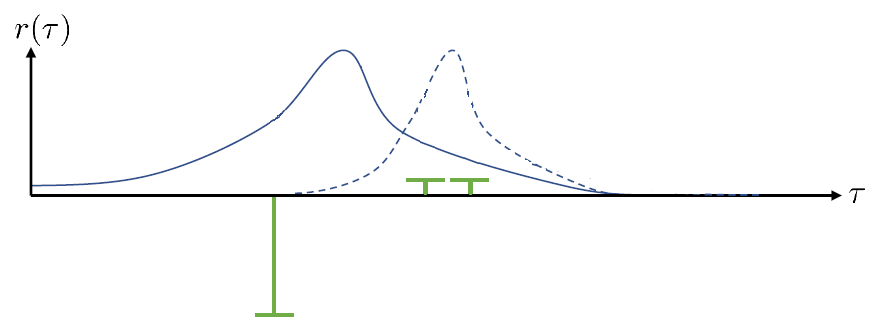
\includegraphics[scale=0.3]{pix/policy/pg_gaussian_reward.png}
%\caption{Histogram of Count Variable}
%\label{fig:label}
\end{figure}
and let's say that I observed three samples, and two 
of those samples had rewards that were small positive numbers, and one sample had a reward 
that was a very negative number. now if I use those three samples just to make my policy 
gradient, you might expect that my policy will kind of slide over to the right a little 
bit, it'll somewhat increase the probability on these two samples and greatly decrease the 
probability on this sample all right, because this sample is a big negative number, so it 
really wants to drive that to a very low probability.

Now let's say that I took that same exact reward function and I added a big constant to it. 
so then my samples would be these yellow lines. the relative rewards are exactly the same. 
All I did is I added a constant, adding a constant doesn't actually change which policy is 
good or bad, because all the constant effects all policies equally, but the policy gradient 
obtained from these rewards will be very different, because now the policy is trying to 
make this more probable, and this even more probable. So it'll actually spread out a little 
bit to cover all three of those things. 

\begin{figure}[h]
\centering
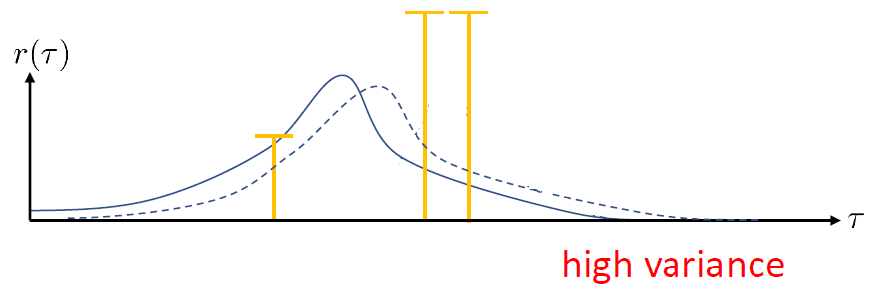
\includegraphics[scale=0.3]{pix/policy/pg_partial_observability_add_big_constant.png}
%\caption{Histogram of Count Variable}
%\label{fig:label}
\end{figure}
and this should be very weird to us, because we haven't actually changed the problem. we 
just added a constant to the objective function, and suddenly our gradient estimate does 
something totally different. As a thought exercise what if the two good samples, these two 
over here actually have a reward of zero, so what if I were to choose the constants, I 
said these two drive down to zero, and this one becomes a big negative number, what might 
happen then, well the distributing thing then is that the direction of the policy goes 
depends entirely with us it starts off on the left side or the right side of this bad 
sample, if it starts off on the left will actually run away from the good stuff, if it 
starts off on the right it'll go towards it. this is a kind of one illustrative example 
of to explain how the policy gradient has high variance, meaning that when you get 
different samples, you get very different gradient estimates from those different samples. 
So for a small finite number of samples, you might get very different policy gradients, 
if you test multiple sample batches. and this is a big problem, because it if in effect 
it means that you're gradient is very noisy. So if you estimate your gradient with a 
modest number of samples, you won't go straight to the optimum, you'll take a really 
zigzag path, and for too large of a learning rate, you might never get there, and this 
is a really big problem for using the policy gradient in practice.


%+++++++++++++++++++++++++++++++++++++++++++
\section{Reducing variance}
%-------------------------------------------

So we'll talk about reducing variance in policy gradients. 
\begin{align*}
\nabla_\theta J(\theta) 
\approx \frac{1}{N}\sum_{i=1}^N
\left( \sum_{t=1}^T \nabla_\theta\log p_\theta(a_{i,t}|s_{i,t}) \right)
\left( \sum_{t=1}^T r(s_{i,t}, a_{i,t}) \right)
\end{align}
The first method that we'll 
use to reduce variance is going to be by exploiting the fact that our universe has 
causality, meaning that the past influences the future, where the future does not influence 
the past. turns out that this particular truth can allow us to get a lower variance policy 
gradient. Why is that well the variance of some quantity is intuitively that the variance 
is bigger if the quantity is bigger, the variance is smaller if the quantity is smaller. 
So if I were to take all these rewards, and make them ten times smaller, numerically the 
variance would also be smaller. that's maybe not super satisfying, but let's see what 
happens when we make use of causality. so more formally here we can say that it means that 
the policy at time $t'$ cannot affect the reward at time $t$, when $t$ is less than $t'$. 
\begin{emp_box}
{\emph Causality}: policy at time $t'$ cannot affect reward at time $t$ when $t < t'$
\end{emp_box}
\noindent
So what you do tomorrow is not going to change what grade you get on the homework tonight.
right because tomorrow it'll be too late unless you take a light day. so here's how we can
use that.
So here we can take this sum over reward and we can distribute it inside the sum over the 
log pi, 
\begin{align*}
\nabla_\theta J(\theta) 
\approx \frac{1}{N}\sum_{i=1}^N
\underset{\textcolor{red}{\xhookleftarrow{\text{\qquad\qquad distribute inside}}}}{
\left( \overset{\textcolor{blue}{\text{sum over }\log p_\theta}}{
\textcolor{blue}{\sum_{t=1}^T \nabla_\theta\log p_\theta(a_{i,t}|s_{i,t})}} \right)
\overset{\textcolor{green}{\text{sum over reward}}}{
\textcolor{green}{\left( \sum_{t=1}^T r(s_{i,t}, a_{i,t}) \right)} }
}
\end{align}
So what I wrote here is just exactly the same as up here, I just use the 
distributive property to distribute this sum over the reward inside of this sum over grad 
log pi. 
\begin{align*}
\nabla_\theta J(\theta) 
\approx \frac{1}{N}\sum_{i=1}^N
\sum_{t=1}^T \nabla_\theta\log p_\theta(a_{i,t}|s_{i,t})
\left( \sum_{t'=1}^T r(s_{i,t'}, a_{i,t'}) \right)
\end{align}
So now I have an outer sum over all the time steps of the grad log pi, times an 
inner sum over $t'$ from $1$ to $T$.
\begin{align*}
\nabla_\theta J(\theta) 
\approx \frac{1}{N}\sum_{i=1}^N
\sum_{t=1}^T \nabla_\theta\log p_\theta(a_{i,t}|s_{i,t})
\left( \sum_{t'=\textcolor{green}{\textcircled{\textcolor{red}{t}}}}^T r(s_{i,t'}, a_{i,t'}) \right)
\end{align}
And now here I can actually make use of causality, because here I have the grad log 
probability of the action at time $t$, but it's being multiplied by a bunch of rewards 
that include reward that happen after $t$, and rewards that happen before $t$. but I 
know that the action that I take a time step $t$ cannot affect the reward at some other 
step $t'$ that happened prior to that. So I can actually make use of this fact to 
change the sum over reward, and what I'm going to do is I'm going to change this number, 
this $1$ to $T$, I'm gonna say when we multiply grad log $p$ it's some time step $t$, 
let's only multiply it by the rewards that we get at that time step and later rather 
than all of the earlier rewards, because it can't affect the earlier rewards. it 
turns out that this is still an unbiased estimator for the policy gradient. and I like 
to show a paper reference at the end of this section, if you want to read more about 
that, but the intuition behind it is that it's basically making use of the fact that 
the action you choose now will not affect the rewards that you got in the past. and the 
reason that this reduces your variance is that now you're multiplying these grad log $p$'s 
by numbers, by sums that are smaller, because you're not adding in all those older 
rewards. So simply by the fact that these sums are now smaller numbers, the overall 
variance of the policy gradient actually goes down. and in practice this little trick is 
very useful for reducing the variance of the policy gradient, and tends to make it work 
quite a lot better.

In fact, it work so much better, that you will often see standard derivations of policy 
gradient, that say that they don't look like this, but instead they use the term reward 
to go often denoted with $Q$\_hat.
\begin{align}
\label{eq_pg_on_policy}
\nabla_\theta J(\theta) 
\approx \frac{1}{N}\sum_{i=1}^N
\sum_{t=1}^T \nabla_\theta\log p_\theta(a_{i,t}|s_{i,t})
\hat{Q}_{i,t}
\end{align}
and they're written like this, they just say grad log $p$ times the {\bf reward to go}. 
And that reward to go hiding inside of there is that sum from time step t until the end, 
representing the total reward that you'll get from that time step until the end of time. 
So this is the actual kind of little more realistic form of the policy gradient that 
you'll often see written out, and you'll often see actually implemented, because there's 
basically no benefit to adding all those rewards from previous time steps, your current 
action cannot affect them, and they only serve to increase the variance.

%+++++++++++++++++++++++++++++++++++++++++++
\subsection{Baselines}

So that's just a neat little trick that basically you should always do, because it never 
hurts and only helps, there's another trick that never hurts and only helps, but it's a 
little bit more involved, in this one we will actually go into in a bit more detail, and 
that's the baseline. So if you remember we had this intuition about how the policy 
gradient works that, it makes the good stuff more likely, and the bad stuff less likely. 
and that was very natural and very appealing, but it's not really true right. 
\begin{align}
%\label{eq_pg_compare_to_mle}
\label{eq_pg_baselines_1}
\nabla_\theta J(\theta) 
\approx \frac{1}{N}\sum_{i=1}^N
\nabla_\theta\log p_\theta(\tau)
r(\tau)
\end{align}
(上式即是前面的公式(\ref{eq_pg_compare_to_mle}),不过我们为了美观将$R$改为了$r$)imagine 
that all of my rewards are like on the order of 1 million, and the good stuff is 1 million 
add 1, and the bad stuff is 1 million minus 1, now the reward are all about 1 million, 
so everything is getting more likely both the good stuff and the bad stuff. so intuitively 
what I would like to do is I'd like to take the things that are better than average, and 
make those more likely, and take the stuff that is worse than average, and make that less 
likely.

\begin{align}
%\label{eq_pg_compare_to_mle}
%\label{eq_pg_baselines_1}
\label{eq_pg_baselines_2}
\nabla_\theta J(\theta) 
&\approx \frac{1}{N}\sum_{i=1}^N \nabla_\theta\log p_\theta(\tau) [r(\tau) - b] \\
b &= \frac{1}{N}\sum_{i=1}^N r(\tau)
\end{align}
yeah like what if we just do that, just take $R(\tau)$(如前,我们为了美观将 $R$ 改为了 $r$) 
and subtract the average reward 
over the samples. So instead of multiplying grad log $p$ by the total reward of that 
trajectory, multiplied by how much better that trajectory is than average, that kind of 
seems very natural, it seems right, like it actually implements trial and error learning, 
but are we actually allowed to do that like? Is that mathematically correct? Well it 
turns out that actually, in expectation this quantity is the same as the one that we had 
before, but has lower variance.

We're going to analyze this new term that we've added right. So all we've done we can 
use again, the distributive property ensure this (grad log $p$ times $R$) minus (grad 
log $p$ times $b$), and let's analyze this grad log $p$ times $b$ term right.

We have an expectation over tau on the outside, what is the expectation of grad log PI 
times $b$. 
$$
\mathbb{E}[\nabla_\theta\log p_\theta(\tau)b]
$$
So we know we never have an expectation you want to know what it means write out the 
actual integral or sum. so we have this integral pi(tau)* grad log p(tau)* b. 
$$
\mathbb{E}[\nabla_\theta\log p_\theta(\tau)b] 
= \int p_\theta(\tau) \nabla_\theta\log p_\theta(\tau)b d\tau
$$
And now we'll go back to our convenient identity equation (\ref{eq_convenient_identity}), 
and let's apply it in Reverse. So before we had to unpack the gradient take out that 
log and take out that $p$. now we're going to pack it back up to take our $p$ times grad 
log $p$ and pack it back into a grad $p$. So now we have grad pi times $b$. 
$$
\mathbb{E}[\nabla_\theta\log p_\theta(\tau)b] 
= \int p_\theta(\tau) \nabla_\theta\log p_\theta(\tau)b d\tau
= \int \nabla_\theta p_\theta(\tau)b d\tau
$$
Now remember the gradient operator commutes with the integration operator. So we can take 
the $b$ on the outside. And we can take the grad on the outside, so we have $b$ times the 
gradient of the integral over tau of $p$ tau. 
$$
\mathbb{E}[\nabla_\theta\log p_\theta(\tau)b] 
= \int p_\theta(\tau) \nabla_\theta\log p_\theta(\tau)b d\tau
= \int \nabla_\theta p_\theta(\tau)b d\tau
= b \nabla_\theta \int p_\theta(\tau) d\tau
$$
What this integral is? Equal to one. Yeah if you integrate a probability distribution, you 
get one, unless you made a coding mistake. So if you implemented it correctly, you should 
get one. And the gradient of one very easy to calculate you don't need a calculus textbook 
for that, that's just zero. So $b$ times grad 1 is 0, which means this whole thing on the 
left is 0. 
$$
\mathbb{E}[\nabla_\theta\log p_\theta(\tau)b] 
= \int p_\theta(\tau) \nabla_\theta\log p_\theta(\tau)b d\tau
= \int \nabla_\theta p_\theta(\tau)b d\tau
= b \nabla_\theta \int p_\theta(\tau) d\tau
= b \nabla_\theta 1
= 0
$$
Which means that you can subtract any constant you want, and you will not change the 
expected policy gradient.

{\bf Q:} Why do we need $b$? 

{\bf A:} So the intuition is you need $b$, so that the good stuff becomes more likely, and 
the bad stuff becomes less likely. The formal reason will be shown later this section. 

So subtracting any $b$ you want, will not change the expectation of the Policy gradient. 
It will however change the variance. So the expectations, the first moment is unaffected. 
The second moment actually is affected. So subtracting baselines is unbiased and 
expectation. It has this nice intuition, that it actually increases the probability of 
things that are better than average, decreases the probability of things that are worse 
than average. 

I'll tell you right now the average reward is not the optimal baseline, but it's pretty 
good. And if you want to implement a baseline in practice, use average reward. But if 
you want to do a bunch of math, then stay with me for the next part. we're going to 
actually derive the optimal baseline.


%+++++++++++++++++++++++++++++++++++++++++++
\subsection{Analyzing variance}

So subtracting a bias does not change the first moment, it does not change the expected 
policy gradient, it does however change the variance. So let's try to figure out what 
that is. Here's the variance equation:
\begin{align}
\operatorname{Var}[x] = \mathbb{E}[x^2] - E[x]^2
\end{align}
and you can just substitute that in, you can take the thing that we want, 
which is our policy gradient, plug that in there. and we're going to try to write out 
the variance of the policy gradient, and then we'll take the derivative of the variance 
with respect to the baseline $b$, set that derivative to $0$, and figure out what the 
optimal baseline is.
\begin{align}
\nabla_\theta J(\theta) = \mathbb{E}_{\tau\sim p_\theta(\tau)}
[\nabla_\theta\log p_\theta(\tau)(r(\tau) - b)]
\end{align}
So let's go on that journey. This is the thing that we're gonna plug in for $x$. 
\begin{align}
\operatorname{Var} = 
\mathbb{E}_{\tau\sim p_\theta(\tau)}
\left[\left(\nabla_\theta\log p_\theta(\tau)(r(\tau) - b)\right)^2\right] - 
\mathbb{E}_{\tau\sim p_\theta(\tau)}
\left[ \nabla_\theta\log p_\theta(\tau)(r(\tau) - b) \right]^2
\end{align}
So here all I've done is I've substituted this in here. So the variance of my policy 
gradient is the expectation under $p_\theta(\tau)$(p theta of tau) of the stuff inside 
the expectation squared, minus the whole expectation with a square on the outside.

Now for that second term, I've already told you that the expectation with the $b$ 
subtracted is exactly the same as the original expectation, that was what I proved 
on the previous subsection. So the second term it's derivative with respect to $b$ is 
going to go to zero:
\begin{align}
\operatorname{Var} = 
\mathbb{E}_{\tau\sim p_\theta(\tau)}
\left[\left(\nabla_\theta\log p_\theta(\tau)(r(\tau) - b)\right)^2\right] - 
\mathbb{E}_{\tau\sim p_\theta(\tau)}&
\underbrace{\left[ \nabla_\theta\log p_\theta(\tau)(r(\tau) - b) \right]^2}_{
\text{this bit is just}\; \mathbb{E}_{\tau\sim p_\theta(\tau)}
[\nabla_\theta\log p_\theta(\tau)r(\tau)]} \\
&\text{(baselines are unbiased in expectation)} \notag
\end{align}
Because it doesn't depend on $b$, so this bit is just the expectation 
squaring it doesn't do anything. So {\bf in terms of its dependence on $b$, so I can just 
ignore that second term, if I want to analyze the effect of $b$ on the variances}.

So it's really only the first term that matters. So I'm gonna change my notation a little 
bit, so that this is a little bit less cluttered, 
\begin{align*}
\frac{d\operatorname{Var}}{db} = \frac{d}{db}
\mathbb{E}\left[g(\tau)^2(r(\tau) - b)^2\right]
\end{align}
I use $g(\tau)$ to denote $\nabla_\theta\log p_\theta(\tau)$. And now I'm going to expand 
it. I'm gonna take that square, I'm going to distribute it inside, and then I'll distribute 
the square inside this difference, and I'm gonna taking the derivative of this whole thing 
with respect to $b$. 
\begin{align*}
\frac{d\operatorname{Var}}{db} = \frac{d}{db}
\mathbb{E}\left[g(\tau)^2(r(\tau) - b)^2\right]
\end{align}
So when I distribute the square, I get three terms, so I have 
d /db( E[ g2 r2 ]- 2* E[ g2 r b] + b2 *E[g2]). So these are the terms that you get, 
with respect to $b$. 
\begin{align*}
\frac{d\operatorname{Var}}{db} 
&= \frac{d}{db}
\mathbb{E}\left[g(\tau)^2(r(\tau) - b)^2\right] \\
&= \frac{d}{db} \left( \mathbb{E}\left[ g(\tau)^2 r(\tau)^2 \right]
- 2 \mathbb{E}\left[ g(\tau)^2 r(\tau) b \right]
+ b^2 \mathbb{E}\left[ g(\tau)^2 \right]
\right)
\end{align}
So now let's look at the derivative of each of these three terms with respect to $b$. For 
the first one, it's zero , because there's no $b$ in there. For the second one, it's just 
it's linear in $b$, so it's just - 2* E[ g2 r ]. and for the third one, it's 2b *E[g2]).
\begin{align*}
\frac{d\operatorname{Var}}{db} 
&= \frac{d}{db}
\mathbb{E}\left[g(\tau)^2(r(\tau) - b)^2\right] \\
&= \frac{d}{db} \left( \cancel{\mathbb{E}\left[ g(\tau)^2 r(\tau)^2 \right]}
- 2 \mathbb{E}\left[ g(\tau)^2 r(\tau) b \right]
+ b^2 \mathbb{E}\left[ g(\tau)^2 \right] \right) \\
&= - 2 \mathbb{E}\left[ g(\tau)^2 r(\tau) \right]
+ 2b \mathbb{E}\left[ g(\tau)^2 \right] \\
&= 0
\end{align}
And I'm going to set this derivative to zero, because I want to find the optimal $b$. 
So when I said to zero, I just have to throw this $-2$ on the right-hand side, divided by 
the first term, and I get an equation for $b$ which says:
\begin{align*}
b = \frac{\mathbb{E}\left[ g(\tau)^2 r(\tau) \right]}{\mathbb{E}\left[ g(\tau)^2 \right]}
\leftarrow \text{This is just expected reward, but weighted by gradient magnitudes!}
\end{align}
And now this thing actually looks an awful lot {\bf like expected reward except I don't 
average the rewards together}. I {\bf instead weight them by their squared gradient}, so 
this is just {\bf expected reward weighted by gradient magnitude}. Now your gradient is 
a vector, it has more than one number in it. And if you actually evaluate this formula, 
$b$ also becomes a vector. You actually get a different baseline value for every entry in 
your gradient depending on the degree to which each trajectory is affected by that parameter 
dimension. 

So you actually get a per dimension baseline if you do this, which is just average reward 
weighted by the magnitude of the gradient for that dimension, and this is the optimal 
baseline, this is the baseline that actually minimizes variance, but if you want to do this 
in practice, my suggestion would be when coding it up, don't bother just use average reward. 
But if you want actually know what the real answer is, this the real answer.

It minimizes variance, I think if you want to get a little bit of intuition for it, it 
basically goes something like this. If that particular dimension is very sensitive, then 
you want to basically emphasize the trajectories, whose probabilities are going to be 
strongly affected by that dimension. So if you have some trajectories that have a very 
high reward, but their probability will not be changed by changing that dimension in 
your parameter vector, then you should not consider them in your baseline. It's kind of 
intuitively somewhat makes sense, but the mathematical reasons that it minimizes variance. 

\noindent
{\bf Q:} So the question is it still optimal, if you also account for the fact that your 
estimate of $b$ will have error do the samples. 

\noindent
{\bf A:}  That's a good question I don't know the answer to that, but yeah maybe we can 
discuss that afterwards.


%+++++++++++++++++++++++++++++++++++++++++++
\subsection{Review}

So let's briefly recap we talked about how the policy gradient has high variance. We 
talked about how we can reduce its variance at essentially no cost by just not adding 
the stuff from the past to the sum. And we talked about baselines which keep the policy 
gradient unbiased, and reduce variance. Let me talk about how we can analyze the variance 
of policy gradient, and use it to drive optional baselines. So in practice if you want 
to get the simplest version of policy gradient that actually works. Definitely use the 
average reward baseline that thing alone will probably do the most to get your policy 
gradient working nicely, then use this causality thing because it's easy and it never 
hurts, and at that point you'll actually get an algorithm that can be used to solve some 
meaningful reinforcement learning problems. So that that's sort of the most basic version 
of policy gradient that actually does something useful, but there's a lot more that 
you could do.

\begin{itemize}
%\setlength{\itemsep}{0pt}
%\setlength{\parsep}{0pt}
\setlength{\parskip}{0pt}
\item
The high variance of policy gradient

\item
Exploiting causality
	\begin{itemize}
	%\setlength{\itemsep}{0pt}
	%\setlength{\parsep}{0pt}
	\setlength{\parskip}{0pt}
	\item[-]
	Future doesn't affect the past
	\end{itemize}

\item
Baselines
	\begin{itemize}
	%\setlength{\itemsep}{0pt}
	%\setlength{\parsep}{0pt}
	\setlength{\parskip}{0pt}
	\item[-]
	Unbiased!
	\end{itemize}

\item
Analyzing variance
	\begin{itemize}
	%\setlength{\itemsep}{0pt}
	%\setlength{\parsep}{0pt}
	\setlength{\parskip}{0pt}
	\item[-]
	Can derive optimal baselines
	\end{itemize}
\end{itemize}


%+++++++++++++++++++++++++++++++++++++++++++
\section{Policy gradient is on-policy}
%-------------------------------------------

In this section, we're going to talk about how the policy gradient is on policy. And 
what we can do about it. So what is on policy mean? {\bf On policy means that every time 
you change your policy, you need to generate new samples, in order to improve your 
policy further.} And you can't reuse old samples that came from other policies, you 
can't even reuse old samples that came from older versions of your own policy. So why 
is that? 
\begin{align*}
\theta^* &= \underset{\theta}{\operatorname{arg max}} J(\theta) \\
J(\theta) &= \mathbb{E}_{\tau\sim p_\theta(\tau)} [r(\tau)] \\
\nabla_\theta J(\theta) =& 
\mathbb{E}_{\tau\sim p_\theta(\tau)}
\left[ \nabla_\theta \log p_\theta(\tau) r(\tau) \right]
\end{align}
Well because the policy gradient is this expectation of $\nabla_\theta \log p_\theta(\tau) r$, 
and the expectation is taken under $p_\theta(\tau)$, and this bit is trouble. 
\begin{align*}
\nabla_\theta J(\theta) &= 
\mathbb{E}_{\underset{\textcolor{blue}{\uparrow}}{\textcolor{red}{\tau\sim p_\theta(\tau)}}}
\left[ \nabla_\theta \log p_\theta(\tau) r(\tau) \right] \\
&\text{\textcolor{blue}{this is trouble}}
\end{align}
It means that every time you want to estimate your gradient, you need to calculate a sample 
wise estimate of an expectation under your current policy. If you apply that gradient and 
change your policy, then you cannot use those same samples to get an unbiased estimate of 
this expectation, because your samples came from now a different distribution. So you now 
generate new samples, so the REINFORCE algorithm which I had before, 
\begin{emp_box}
Loop of REINFORCE algorithm:
\begin{itemize}
%\setlength{\itemsep}{0pt}
%\setlength{\parsep}{0pt}
\setlength{\parskip}{0pt}
\item[1.]
sample $\{\tau^i\}$ from $\pi_\theta(a_t|s_t)$ (run it on the robot) 
\textcolor{red}{$\leftarrow$ can't just skip this!}
\item[2.]
$\nabla_\theta J(\theta) \approx \sum_i(\sum_t\nabla_\theta\log\pi_\theta(a_t^i|s_t^i))
(\sum_tr(s_t^i, a_t^i))$
\item[3.]
$\theta \leftarrow \theta + \alpha\nabla_\theta J(\theta)$
\end{itemize}
\end{emp_box}\noindent
this step one, which is sample your trajectories from your policy, you can't just skip 
that stuff. You have to have it there. If you skip that step, then you're not getting a 
real policy gradient, and your policy may not improve.

Now this is a little bit of a problem when we're doing deep reinforcement learning, 
because neural networks typically change only a little bit with each gradient step. 
In general the more non-linear your function approximator is, the smaller the step 
you'll need, the less it'll change with each gradient step, which means that you might 
need many gradient steps which means that for the REINFORCE algorithm, you might need 
a whole lot of samples. And if those samples are expensive, if they involve, let's say 
driving a real car in the edge of a cliff, you'll need an awful lot of cars in order to 
improve your policy substantially. On policy learning can be extremely inefficient for 
this reason, but that doesn't mean that it's not useful. You might have a setting, where 
you're using a cheap simulator, there it's no problem to generate tons of samples. In 
fact we won't have you driving real cars, we'll have you driving simulated lunar landers, 
and half cheetahs.


%+++++++++++++++++++++++++++++++++++++++++++
\subsection{Off-policy learning & importance sampling}

But there is something that we can do, if we want this method to be more efficient. We can actually turn policy gradients into a somewhat off policy algorithm, it is sort of what I would call textbook off policy. in reality we can debate as to how a policy really is, but in principle this will be an off policy algorithm, and we'll do that using importance sampling.

So what if we don't have samples from $p_\theta(\tau)$, and we still want to do our 
policy gradient. well we say that we have some samples from some other $p_\theta(\tau)$ 
instead, in practice $\bar{p}(\tau)$ would often be a previous version of our policy, 
but it doesn't have to be, it's just some other distribution. And to briefly recap for 
those of you that don't remember what important sampling is. Important sampling is a 
very simple, very convenient technique, that we can use to estimate expectations under 
one distribution when we only have access to samples from a different distribution. So 
if I want to estimate the expectation of $f(x)$ under $p(x)$, 
\begin{align*}
\mathbb{E}_{x\sim p(x)} [f(x)]
\end{align}
again whenever you see expectation you need to actually do some math, get rid of the 
expectation symbol, just write it as an integral. 
\begin{align*}
\mathbb{E}_{x\sim p(x)} [f(x)] = \int p(x) f(x) dx
\end{align}
And now it's very convenient and mathematical, so you can always multiply something by 
one, and not change its value. So that's what we're going to do, we're going to multiply 
it by one, specifically by the one that is equal to $q(x) / q(x)$, and now we'll just 
take this little fraction symbol, and we'll slide it over a little bit to write it like 
following. 
\begin{align*}
\mathbb{E}_{x\sim p(x)} [f(x)] 
&= \int p(x) f(x) dx \\
&= \int \frac{q(x)}{q(x)} p(x) f(x) dx \\
&= \int q(x) \frac{p(x)}{q(x)} f(x) dx
\end{align}
Very nice trick and now it's an integral with a q(X) out front which means that it's an 
expectation under $q(x)$, so the expectation under $p(x)$ of $f(x)$ is equal to the 
expectation under $q(x)$ of $(p(x) / q(x)) * f(x)$. 
\begin{emp_box}
\noindent
importance sampling:
\begin{align*}
\mathbb{E}_{x\sim p(x)} [f(x)] 
&= \int p(x) f(x) dx \\
&= \int \frac{q(x)}{q(x)} p(x) f(x) dx \\
&= \int q(x) \frac{p(x)}{q(x)} f(x) dx \\
&= \mathbb{E}_{x\sim q(x)} \left[ \frac{p(x)}{q(x)} f(x) \right]
\end{align}
\end{emp_box}\noindent
And that's basically the equation for important sampling, it means that if you have 
samples from $q(x)$ just multiply them by the ratio of their probabilities, then multiply 
them by your function value, averaged together your samples, and you will have an 
unbiased estimate of the quantity that you want.

So we can plug that into policy gradient, and bang there, we have our off-policy policy 
gradient. 
\begin{align*}
J(\theta) = \mathbb{E}_{\tau \sim \bar{p}(\tau)}
\left[ \frac{p_\theta(\tau)}{\bar{p}_\theta(\tau)} r(\tau) \right]
\end{align}
Now there's a little bit of a problem though, because you know these these $p_\theta(\tau)$, 
$\bar{p}_\theta(\tau)}$. They contain a bunch of stuff in there that we don't know, 
(see equation (\ref{eq_pg_p_theta_trajectories}))
\begin{equation}
%\label{eq_pg_p_theta_trajectories}
\label{eq_pg_p_theta_trajectories_s}
p_{\theta}(\tau) = p(s_1)
\prod_{t=1}^T p_\theta(a_t|s_t) p(s_{t+1}|s_t, a_t)
\end{equation}
like $p(s_1)$, $p(s_{t+1}|s_t,a_t)$ and so on. So we're not quite ready to implement this 
thing yet. We need to actually unpack this probability and see what it's equal to. So that 
we can make it practical. So remember our trajectory probabilities are given by this 
equation which means that if we write out this ratio, we get this thing. So we have all 
the terms on the top, and all the terms on the bottom, and conveniently enough. 
\begin{align*}
\frac{p_\theta(\tau)}{\bar{p}_\theta(\tau)} =
\frac{\cancel{p(s_1)} \prod_{t=1}^T p_\theta(a_t|s_t) \cancel{p(s_{t+1}|s_t,a_t)}}{
\cancel{p(s_1)} \prod_{t=1}^T \bar{p}_\theta(a_t|s_t) \cancel{p(s_{t+1}|s_t,a_t)}}
= \frac{\prod_{t=1}^T p_\theta(a_t|s_t)}{\prod_{t=1}^T \bar{p}_\theta(a_t|s_t)}
\end{align}
All of the things that we don't know, the $p(s_1)$ and the $p(s_{t+1}|s_t,a_t)$ appear 
on both the top and bottom which means that we can cancel them out. So all we're left with 
is a ratio of the products of the action probabilities under the new policy divided by 
the products of the action probabilities under the old policy, and that's actually 
something we can code up, that's something we can implement. So these are the actual 
importance weights that we have.


%+++++++++++++++++++++++++++++++++++++++++++
\subsection{Deriving the policy gradient with IS}

Now you can actually use important sampling to derive the policy gradients in an 
alternate way, so we had one derivation at the beginning of the lecture, now I'll very 
briefly show a slightly different derivation that uses important sampling. And this kind 
of view of policy gradient will actually be useful later on in subsequent lectures also. 
So let's take our objective value, and let's express our objective value in terms of some 
new parameters $\theta'$. So we can write out $J(\theta')$ as the expectation under 
$p_\theta$ that's our old policy of the importance sampling ratio times $r(\tau)$. 
\begin{align*}
\theta^* &= \underset{\theta}{\operatorname{arg max}} J(\theta) \\
J(\theta) &= \mathbb{E}_{\tau\sim p_\theta(\tau)} [r(\tau)] \\
J(\theta') &= \mathbb{E}_{\tau\sim p_\theta(\tau)} 
\left[ \frac{p_{\theta'}(\tau)}{p_\theta(\tau)} r(\tau) \right] 
\end{align}
And the nice thing about this equation is that $\theta'$ only appears in the numerator 
of this fraction and not in the distribution with respect to which we take the expectation. 
So now when we go to take the gradient of this, we don't even have to worry about how 
we're sampling or what we're sampling from, this is the only bit that depends on $\theta'$. 
So if we write out $\nabla_{\theta'} J(\theta')$ basically just literally take the 
derivative of this quantity up here, we get this,
\begin{align*}
\nabla_{\theta'} J(\theta')  
&= \mathbb{E}_{\tau\sim p_\theta(\tau)}
\left[ \frac{\nabla_{\theta'} p_{\theta'}(\tau)}{p_\theta(\tau)} r(\tau) \right] \\
&= \mathbb{E}_{\tau\sim p_\theta(\tau)}
\left[ \frac{p_{\theta'}(\tau)}{p_\theta(\tau)} 
\nabla_{\theta'} \log p_{\theta'}(\tau) r(\tau) \right]
\end{align}
Then we apply our $\nabla_\theta \log p$ trick again. The convenient identity and we get 
this. and now $\theta'$ appears in the numerator, and it appears over here, and it 
appears nowhere else. So if we want to use this to obtain a formula for the standard 
on-policy policy gradient, that's just the special case of this equation, where $\theta$ 
is equal to $\theta'$. So if we want to estimate the policy gradient locally around the 
current value of the parameters which is $\theta$, then this ratio becomes 1, 
\begin{align*}
\nabla_{\theta'} J(\theta')  
&= \mathbb{E}_{\tau\sim p_\theta(\tau)}
\left[ \frac{\nabla_{\theta'} p_{\theta'}(\tau)}{p_\theta(\tau)} r(\tau) \right] \\
&= \mathbb{E}_{\tau\sim p_\theta(\tau)}
\left[ \frac{\cancel{p_{\theta'}(\tau)}}{\cancel{p_\theta(\tau)}} 
\nabla_{\theta'} \log p_{\theta'}(\tau) r(\tau) \right]
\end{align}
and we get our old familiar policy gradient: 
\begin{align*}
\nabla_\theta J(\theta) = \mathbb{E}_{\tau\sim p_\theta(\tau)}
\left[ \nabla_\theta \log p_\theta(\tau) r(\tau) \right]
\end{align}
So this is an alternative way to derive the policy gradient, starting from important 
sampling without having to worry about how we're sampled whatever or where the sampling 
is always with respect to the old policy. But of course we could also consider the case 
where $\theta$ is not equal to $\theta'$, and then get an actual off-policy policy gradient.


%+++++++++++++++++++++++++++++++++++++++++++
\subsection{The off-policy policy gradient}

So the off policy policy gradient, the same formula, but when $\theta$ is not equal to 
$\theta'$. 
\begin{align*}
\theta^* &= \underset{\theta}{\operatorname{arg max}} J(\theta) \\
J(\theta) &= \mathbb{E}_{\tau\sim p_\theta(\tau)} [r(\tau)] \\
J(\theta') &= \mathbb{E}_{\tau\sim p_\theta(\tau)} 
\left[ \frac{p_{\theta'}(\tau)}{p_\theta(\tau)} r(\tau) \right] \\
\nabla_{\theta'} J(\theta')  
&= \mathbb{E}_{\tau\sim p_\theta(\tau)}
\left[ \frac{p_{\theta'}(\tau)}{p_\theta(\tau)} 
\nabla_{\theta'} \log p_{\theta'}(\tau) r(\tau) \right]
\end{align}
So now we're going to substitute in our equation for the importance weights 
from before, and we get this thing(注意前面的公式(\ref{eq_pg_gradient_of_log_p_trajectory})): 
\begin{align}
\nabla_{\theta'} J(\theta')  
&= \mathbb{E}_{\tau\sim p_\theta(\tau)}
\left[ \frac{p_{\theta'}(\tau)}{p_\theta(\tau)} 
\nabla_{\theta'} \log p_{\theta'}(\tau) r(\tau) \right] \notag\\
&= \mathbb{E}_{\tau\sim p_\theta(\tau)}
\left[ \left( \prod_{t=1}^T\frac{p_{\theta'}(a_t|s_t)}{p_\theta(a_t|s_t)} \right) 
\left( \sum_{t=1}^T \nabla_{\theta'}\log p_{\theta'} (a_t | s_t) \right) 
\left( \sum_{t=1}^T r(s_t, a_t) \right)
\right]
\label{eq_pg_off_policy_deducing}
\end{align}
So before we have two terms, we had the sum over the $\nabla_\theta\log p$, and the 
rewards, now we have three terms, we've also multiplied in the importance weights.

\noindent
{\bf Q:} Why is it a bad idea to do this? What might go wrong with this formula? 
What if T is really big. 

\noindent
{\bf A:} So the intuition here is that these this product you know you have a product 
of ratios, it's the same as a ratio of products, you can put the product on the top, 
and the product on the bottom, and probabilities are numbers between $0$ & $1$. So when 
you take a very large number of numbers between $0$ & $1$ and you multiply them together, 
you get really really small numbers. So you have a really small number on top, and a 
really small number on the bottom. How small will exponentially small, because it's on 
you know if all of your probabilities are on the order of epsilon, both the numerator 
and the denominator are on the order of epsilon to the power $T$. So you take the ratio 
of these things, and you're going to get weights that are either gigantic or tiny, and 
that will do exactly the thing that we least want for our policy gradients which rule 
it'll reach that it will increase the variance. And all that hard work would put into 
designing baselines and so on will be negated by the enormous variance that we'll get 
from those crazy importance weights, that's a big problem for important sample policy 
gradients.
\begin{align*}
\nabla_{\theta'} J(\theta')  
&= \mathbb{E}_{\tau\sim p_\theta(\tau)}
\left[ \left( \prod_{t=1}^T\frac{p_{\theta'}(a_t|s_t)}{p_\theta(a_t|s_t)} \right) 
\left( \sum_{t=1}^T \nabla_{\theta'}\log p_{\theta'} (a_t | s_t) \right) 
\left( \sum_{t=1}^T r(s_t, a_t) \right)
\right] \\
&= \mathbb{E}_{\tau\sim p_\theta(\tau)}
\left[ \sum_{t=1}^T \nabla_{\theta'}\log p_{\theta'} (a_t | s_t)
\left( \prod_{t'=1}^t\frac{p_{\theta'}(a_{t'}|s_{t'})}{p_\theta(a_{t'}|s_{t'})} \right) 
\left( \sum_{t'=t}^T r(s_{t'}, a_{t'}) 
\left( \prod_{t"=t}^{t'}\frac{p_{\theta'}(a_{t"}|s_{t"})}{p_\theta(a_{t"}|s_{t"})} \right)
\right) \right]
%\label{eq_pg_off_policy_deducing}
\end{align}
We can do a few tricks, we can exploit this causality thing, so we can basically take 
this product, and we can put a piece of it inside the reward term, and put the other 
piece over here, and then the rewards can go from $t$ to $T$ instead of $1$ to $T$. 
\begin{align*}
\nabla_{\theta'} J(\theta')  
&= \mathbb{E}_{\tau\sim p_\theta(\tau)}
\left[ \left( \prod_{t=1}^T\frac{p_{\theta'}(a_t|s_t)}{p_\theta(a_t|s_t)} \right) 
\left( \sum_{t=1}^T \nabla_{\theta'}\log p_{\theta'} (a_t | s_t) \right) 
\left( \sum_{t=1}^T r(s_t, a_t) \right)
\right] \\
&= \mathbb{E}_{\tau\sim p_\theta(\tau)}
\left[ \sum_{t=1}^T \nabla_{\theta'}\log p_{\theta'} (a_t | s_t)
\underset{\textcolor{blue}{\uparrow}}{\left( 
\textcolor{red}{\prod_{t'=1}^t\frac{p_{\theta'}(a_{t'}|s_{t'})}{p_\theta(a_{t'}|s_{t'})}} \right)} 
\left( \sum_{t'=t}^T r(s_{t'}, a_{t'}) 
\left( \prod_{t"=t}^{t'}\frac{p_{\theta'}(a_{t"}|s_{t"})}{p_\theta(a_{t"}|s_{t"})} \right)
\right) \right] \\
&\qquad\qquad\qquad\qquad\qquad
\text{\textcolor{blue}{future actions don't affect current weight}}
%\label{eq_pg_off_policy_deducing}
\end{align}
So we can still apply that trick, but we haven't really solved the real problem, which 
is that we're multiplying together all of $T$ different numbers between $0$ and $1$. 
So causality hopefully all of you I've got that picture. Now one thing we can do at this 
point is we could just delete this part of the weights, that will actually change the 
algorithm. So you will not get the same gradient if you do that, but it turns out that 
if you set this part to $1$, you do still get an algorithm where each gradient step will 
improve the policy, but for a different reason. So if you set this part to $1$, you actually 
get a policy iteration algorithm, 
\begin{align*}
\nabla_{\theta'} J(\theta')  
&= \mathbb{E}_{\tau\sim p_\theta(\tau)}
\left[ \left( \prod_{t=1}^T\frac{p_{\theta'}(a_t|s_t)}{p_\theta(a_t|s_t)} \right) 
\left( \sum_{t=1}^T \nabla_{\theta'}\log p_{\theta'} (a_t | s_t) \right) 
\left( \sum_{t=1}^T r(s_t, a_t) \right)
\right] \\
&= \mathbb{E}_{\tau\sim p_\theta(\tau)}
\left[ \sum_{t=1}^T \nabla_{\theta'}\log p_{\theta'} (a_t | s_t)
\left( \prod_{t'=1}^t\frac{p_{\theta'}(a_{t'}|s_{t'})}{p_\theta(a_{t'}|s_{t'})} \right) 
\left( \sum_{t'=t}^T r(s_{t'}, a_{t'}) 
\left( \prod_{t"=t}^{t'}\frac{p_{\theta'}(a_{t"}|s_{t"})}{p_\theta(a_{t"}|s_{t"})} \right)
\right) \right] \\
&= \mathbb{E}_{\tau\sim p_\theta(\tau)}
\left[ \sum_{t=1}^T \nabla_{\theta'}\log p_{\theta'} (a_t | s_t)
\left( \prod_{t'=1}^t\frac{p_{\theta'}(a_{t'}|s_{t'})}{p_\theta(a_{t'}|s_{t'})} \right) 
\left( \sum_{t'=t}^T r(s_{t'}, a_{t'}) 
\underset{\textcolor{blue}{\uparrow}}{\left( \xcancel{
\prod_{t"=t}^{t'}\frac{p_{\theta'}(a_{t"}|s_{t"})}{p_\theta(a_{t"}|s_{t"})}} \right)}
\right) \right] \\
&\qquad\qquad\qquad\qquad\qquad\qquad\qquad\qquad\qquad\qquad\qquad\qquad\qquad
\text{\textcolor{blue}{if we ignore this, we get }} \\
&\qquad\qquad\qquad\qquad\qquad\qquad\qquad\qquad\qquad\qquad\qquad\qquad\quad
\text{\textcolor{blue}{a policy iteration algorithm }} \\
&\qquad\qquad\qquad\qquad\qquad\qquad\qquad\qquad\qquad\qquad\qquad\qquad
\text{\textcolor{blue}{(more on this later in this chapter)}} 
%\label{eq_pg_off_policy_deducing}
\end{align}
And we'll cover policy iteration later on in this chapter, but you can't actually show 
that setting this bit to one will allow you to still improve your policy, but for a 
different reasons. 

So the policy gradient will not be equal to the old policy gradient, but the policy will 
still improve, and that we'll cover later on when we talk about policy iteration. but even 
after doing that you're still left with this piece, and this is still a product of $O$(
$T$ numbers between $0$ and $1$). So we're still in trouble.


%+++++++++++++++++++++++++++++++++++++++++++
\subsection{A first-order approximation for IS}

\begin{align*}
\nabla_{\theta'} J(\theta')  
= \mathbb{E}_{\tau\sim p_\theta(\tau)}
\left[ \sum_{t=1}^T \nabla_{\theta'}\log p_{\theta'} (a_t | s_t)
\left( \prod_{t'=1}^t\frac{p_{\theta'}(a_{t'}|s_{t'})}{p_\theta(a_{t'}|s_{t'})} \right) 
\left( \sum_{t'=t}^T r(s_{t'}, a_{t'}) \right) \right] 
%\label{eq_pg_off_policy_deducing}
\end{align}
So here is one somewhat hand-waving thing we can do, it'll be hand waving today, it'll 
be less hand waving in the second half of the chapter. So what we can do is we can employ 
a kind of a first order approximation. And you'll understand order approximation in a 
subsequent lecture, but for now I just want to tell you what it is, just so if you have 
to implement it, you'll know the general idea. 
\begin{align*}
\nabla_{\theta'} J(\theta')  
&= \mathbb{E}_{\tau\sim p_\theta(\tau)}
\left[ \sum_{t=1}^T \nabla_{\theta'}\log p_{\theta'} (a_t | s_t)
\underset{\textcolor{blue}{\uparrow}}{\left( 
\textcolor{red}{\prod_{t'=1}^t\frac{p_{\theta'}(a_{t'}|s_{t'})}{p_\theta(a_{t'}|s_{t'})}} \right)} 
\left( \sum_{t'=t}^T r(s_{t'}, a_{t'}) \right) \right] \\
&\qquad\qquad\qquad\qquad\qquad\qquad\qquad\qquad
\textcolor{blue}{\text{exponential in }T\ldots} 
%\label{eq_pg_off_policy_deducing}
\end{align}
So this red bit is still exponential in $T$, and we're very unhappy about that. So let's 
write the objective a little bit differently.
Here is our on-policy policy gradient from equation (\ref{eq_pg_on_policy}), 
\begin{align*}
%\label{eq_pg_on_policy}
&\text{on-policy policy gradient:} \\
&\nabla_\theta J(\theta) 
\approx \frac{1}{N}\sum_{i=1}^N
\sum_{t=1}^T \nabla_\theta\log 
\textcolor{red}{p_\theta(a_{i,t}\underset{\textcolor{blue}{\uparrow}}{|}s_{i,t})}
\hat{Q}_{i,t} \\
&\qquad\qquad\qquad\qquad\qquad\qquad
\textcolor{blue}{(s_{i,t},a_{i,t}) \sim p_\theta(s_t,a_t)} 
\end{align}
\noindent
and this on-policy policy gradient, here I wrote it in this kind of reward to go form 
using the $Q$ hat from before. This on policy policy gradient requires us to sample these 
$s_{i,t}$ and $a_{i,t}$ from the state action marginal, remember the state action marginal 
from last chapter. Here it doesn't actually matter that these $s_{i,t}$'s and $a_{i,t}$'s 
come from the same trajectory or not, they're just multiplied by the reward to go so long 
as they come from the state action marginal, we're happy, which means that we can write 
the off-policy policy gradient with importance weights a little bit differently. we can 
write it with the importance weights given by the ratio of state action marginal probabilities.
\begin{align*}
%\label{eq_pg_on_policy}
&\text{off-policy policy gradient:} \\
&\nabla_{\theta'} J(\theta') \\
&\approx \frac{1}{N}\sum_{i=1}^N
\sum_{t=1}^T \frac{p_{\theta'}(s_{i,t},a_{i,t})}{p_\theta(s_{i,t},a_{i,t})}
\nabla_{\theta'}\log p_{\theta'}(a_{i,t}|s_{i,t}) \hat{Q}_{i,t}
\end{align}
\noindent
so we have $p_{\theta'}(a_{i,t}|s_{i,t})/p_\theta(s_{i,t},a_{i,t})$. Now there's still a 
bit problematic, because we don't know what the state action marginals are, we just have 
a policy. But that doesn't stop us from factorizing this using the chain rule into a 
product of two terms, the policy term which we're all familiar with, and this really 
annoying state marginal term. We have no idea what the state marginals are, but what we 
can do is we can sort of embrace our ignorance there, and just ignore that part. 
\begin{align*}
%\label{eq_pg_on_policy}
&\text{off-policy policy gradient:} \\
&\nabla_{\theta'} J(\theta') \\
&\approx \frac{1}{N}\sum_{i=1}^N
\sum_{t=1}^T \frac{p_{\theta'}(s_{i,t},a_{i,t})}{p_\theta(s_{i,t},a_{i,t})}
\nabla_{\theta'}\log p_{\theta'}(a_{i,t}|s_{i,t}) \hat{Q}_{i,t} \\
&= \frac{1}{N}\sum_{i=1}^N \sum_{t=1}^T 
\underset{\textcolor{blue}{\uparrow}}{\cancel{ \frac{p_{\theta'}(s_{i,t})}{p_\theta(s_{i,t})} }}
\frac{p_{\theta'}(a_{i,t} | s_{i,t})}{p_\theta(a_{i,t} | s_{i,t})}
\nabla_{\theta'}\log p_{\theta'}(a_{i,t}|s_{i,t}) \hat{Q}_{i,t} \\
&\qquad\qquad\qquad
\textcolor{blue}{\text{ignore this part}} 
\end{align}
\noindent
And this will actually work, if $\theta'$ is close to $θ$, we'll find out why this works 
later in this chapter, when we talk about advanced policy gradients. But you can actually 
show that when theta and theta prime are close enough to each other, the error that you get 
from deleting this term is small. For now you'll have to take my word for it, but if you 
want to actually implement important sample policy gradient in practice, please don't do 
this. I made that mistaken in one of my paper several years ago(2013), do this instead 
will work much better. and then you'll find out why it's actually okay to do later on.

This is just basically using importance sampling to estimate this quantity, so this quantity 
is the policy gradient, whenever $s_{i,t}$ and $a_{i,t}$ are drawn from the state action 
marginal, i mean it's true whenever they're drawn from a trajectory distribution, but 
because only the state action marginal lecture depends on $s_t$, $a_t$, you can say well 
instead of putting in $p_\theta(\tau)$ here just put in p_\theta(s_t,a_t)$, because that's 
the only thing that depends on the state and action at time $t$. and once you know that, 
then you can do the same exact important sampling that we did before for trajectories, 
only now at the level of state action marginals, ordinarily this wouldn't be very useful, 
because we don't know what the state action marginals are, but if we just delete the 
state part, then we have two terms that we do understand, and that that's something we 
can implement. Well so the version that you would implement is this thing, so you cannot 
implement this part, because evaluating state marginals is extremely difficult. so you 
would not implement this, you would just implement this.

yes precisely if we look at the KL divergence of theta, yes so so as sort of a preview for a lecture four weeks from now. yes the this this thing is okay to do, if the KL divergence between πθ’ and πθ is small. yes right so the question is why are we doing all this stuff, the reason we're doing this is so that in the off policy setting, as you said we can include more samples in our sample wise estimate, because variance is high which means that we want lots of samples to get a good estimate. we can't use samples from old policies, unless we do something like important sampling, so in practice the effective number of samples we can utilize becomes much larger. So this is a slightly more complex question, so the question for those of you that didn't hear is, are we only allowed to use samples from our own previous policies or can we use samples from somewhere else. It depends on which formula we're talking about, so if we go back here this thing, this thing you can do for any old policy or anybody else's policy, so any policy can be plugin in place of pi theta into this formula, and that will be correct. the bit where I killed the this ratio that does assume that pi theta was my own old policy, so there I'm actually making that assumption, but if I don't kill that part, I can use any policy I want. if you're doing this thing, and actually deleting the state probabilities, this you should only do when PI theta is a recent old policy, because you need PI theta and PI theta prime to be close together.



%+++++++++++++++++++++++++++++++++++++++++++
\subsection{Policy gradient with automatic differentiation}




%+++++++++++++++++++++++++++++++++++++++++++
\subsection{Policy gradient in pratice}



%+++++++++++++++++++++++++++++++++++++++++++
\subsection{Review}

Brief review and then I'll conclude the policy gradient is an on-policy method, You 
can derive an off policy variant using important sampling. The importance weights have 
exponential scaling in $T$. You can ignore parts of the weights which gives you an 
approximation which we're now it looks like a hack, but later on we'll see that it 
actually makes some mathematical sense, and you can implement it with automatic 
differentiation software, but you have to be a little careful to make sure that you 
don't naively just compute out all the $\nabla_\theta\log p$ and instead ask your audit 
if software to do it for you. 
\begin{itemize}
%\setlength{\itemsep}{0pt}
%\setlength{\parsep}{0pt}
\setlength{\parskip}{0pt}
\item
Policy gradient is on-policy

\item
Can derive off-policy variant
	\begin{itemize}
	%\setlength{\itemsep}{0pt}
	%\setlength{\parsep}{0pt}
	\setlength{\parskip}{0pt}
	\item[-]
	Use importance sampling

	\item[-]
	Exponential scaling in $T$

	\item[-]
	Can ignore state portion (approximation)
	\end{itemize}

\item
Can implement with automatic differentiation - need to know what to backpropagate

\item
Practical considerations: batch size, learning rates, optimizers
\end{itemize}


%+++++++++++++++++++++++++++++++++++++++++++
\section{Is the Policy Gradient a Gradient?}
%-------------------------------------------
% https://all.cs.umass.edu/pubs/2020/Nota%20and%20Thomas%20-%20Is%20the%20Policy%20Gradient%20a%20Gradient.pdf


$\mathfrak{a}$

